\documentclass[10pt]{beamer}
\usepackage{bm}

\usetheme[progressbar=frametitle,sectionpage=progressbar]{metropolis}
\usepackage{appendixnumberbeamer}

\usepackage{booktabs}
\usepackage[scale=2]{ccicons}

\usepackage{pdfpages}
\usepackage{pgfplots}
\usepgfplotslibrary{dateplot}

\usepackage[utf8]{inputenc} % usually not needed (loaded by default)

\usepackage{xspace}
\newcommand{\themename}{\textbf{\textsc{metropolis}}\xspace}

\usepackage{media9}
\usepackage[export]{adjustbox}

\title{Hero Net Interpreter}
\subtitle{Final presentation}
\date{\today}
% \date{}
\author{Martin Jérémie}
\institute{University of Geneva}
% \titlegraphic{\hfill\includegraphics[height=1.5cm]{logo.pdf}}

\usepackage[labelformat=empty]{caption}

\usepackage[ruled,vlined]{algorithm2e}
\usepackage{algpseudocode}% http://ctan.org/pkg/algorithmicx
\usepackage{varwidth}% http://ctan.org/pkg/varwidth

\begin{document}

\maketitle

\section{Hero net foundations}

\begin{frame}[fragile]{From Predicate nets...}
    \begin{figure}
        \centering
        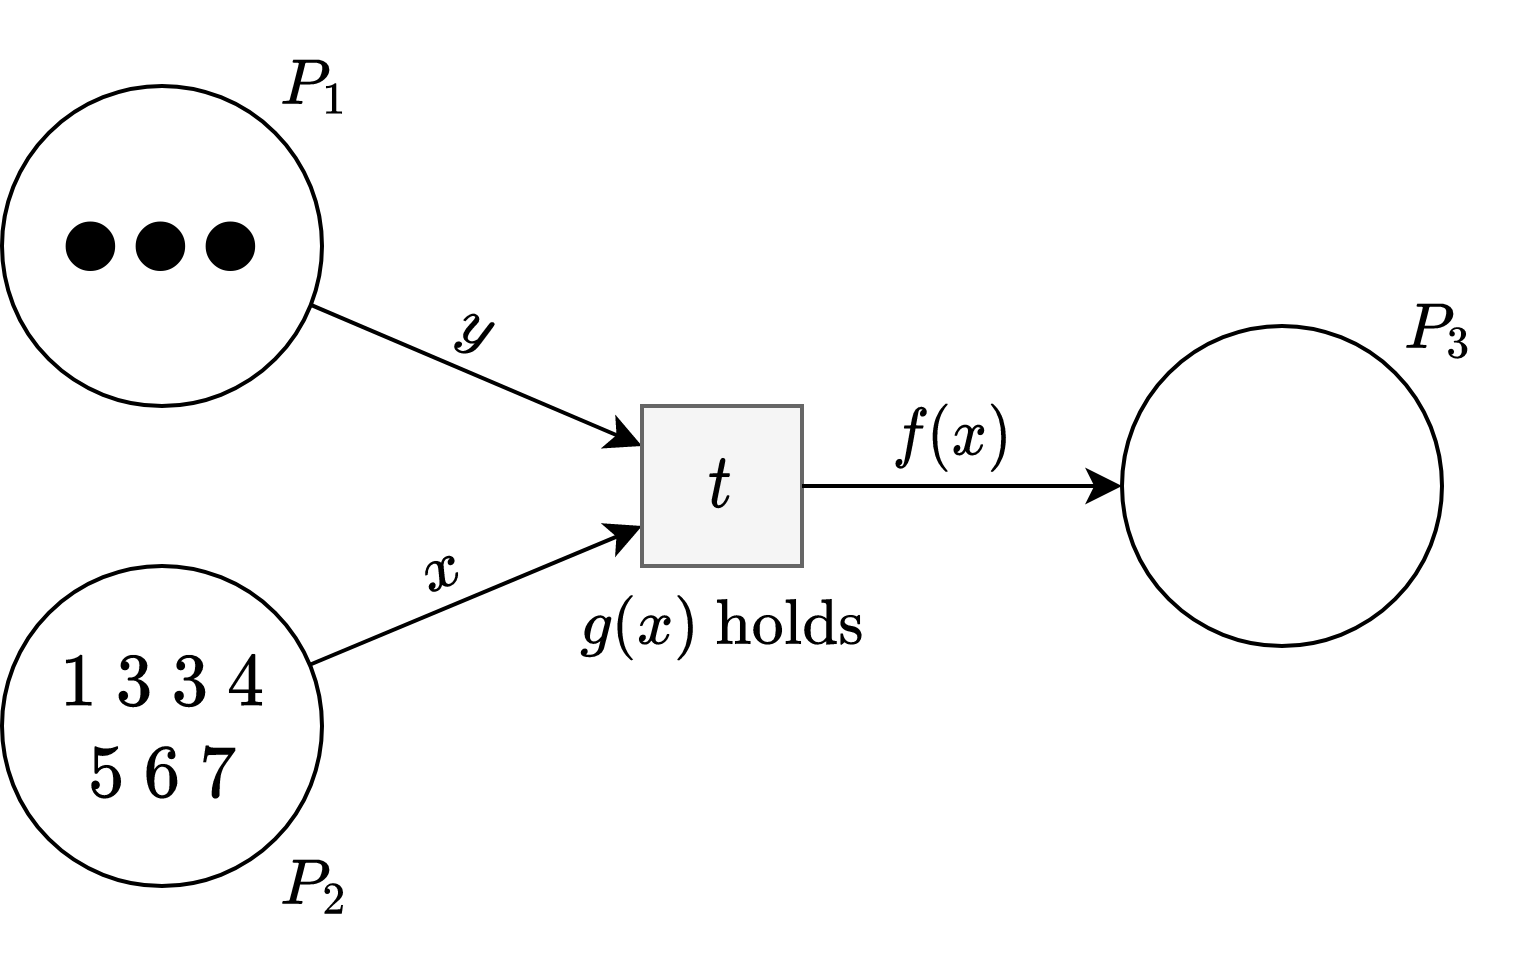
\includegraphics[width=0.8\textwidth]{01petri.png}
    \end{figure}
    \begin{itemize}
        \item How to model and execute \textbf{Hero nets}?
        \item Started with a library for \textit{Predicate Nets}
    \end{itemize}
\end{frame}

\begin{frame}[fragile]{... to Hero nets}
    \begin{figure}
        \centering
        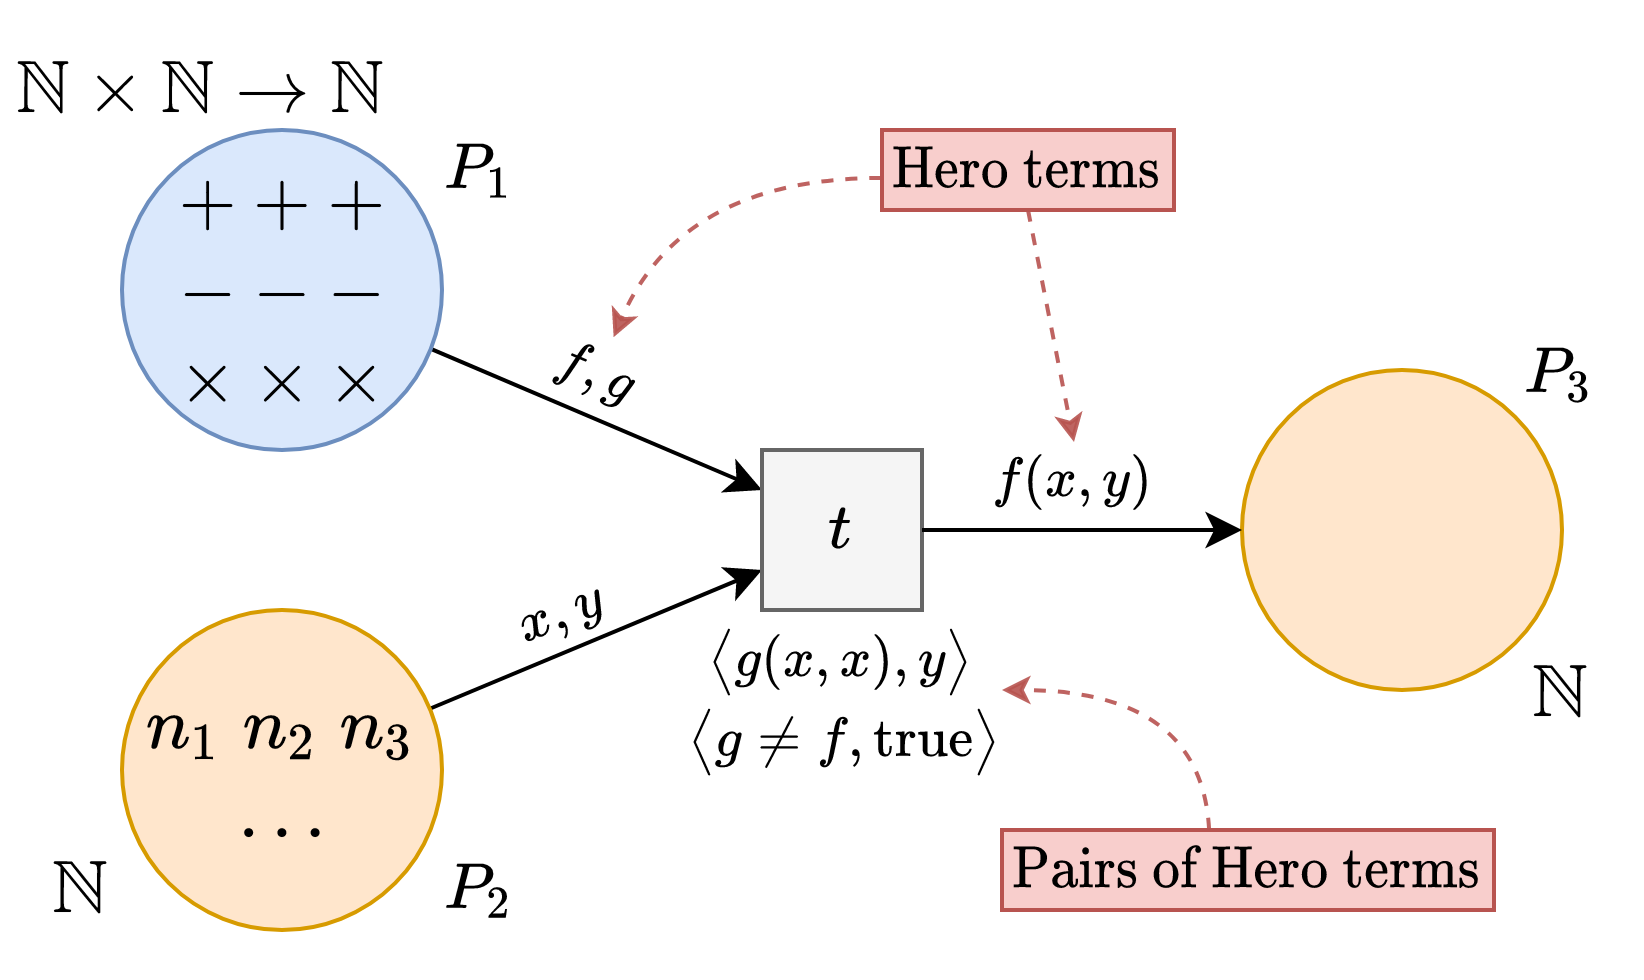
\includegraphics[width=0.80\textwidth]{02heronet.png}
    \end{figure}
    \begin{itemize}
        \item Token: set of values
        \item Transition arc: multiset of Hero terms
        \item Guard: set of pairs of Hero terms
    \end{itemize}
\end{frame}

\begin{frame}[fragile]{Alpine integration with Hero nets}
    \begin{figure}
        \centering
        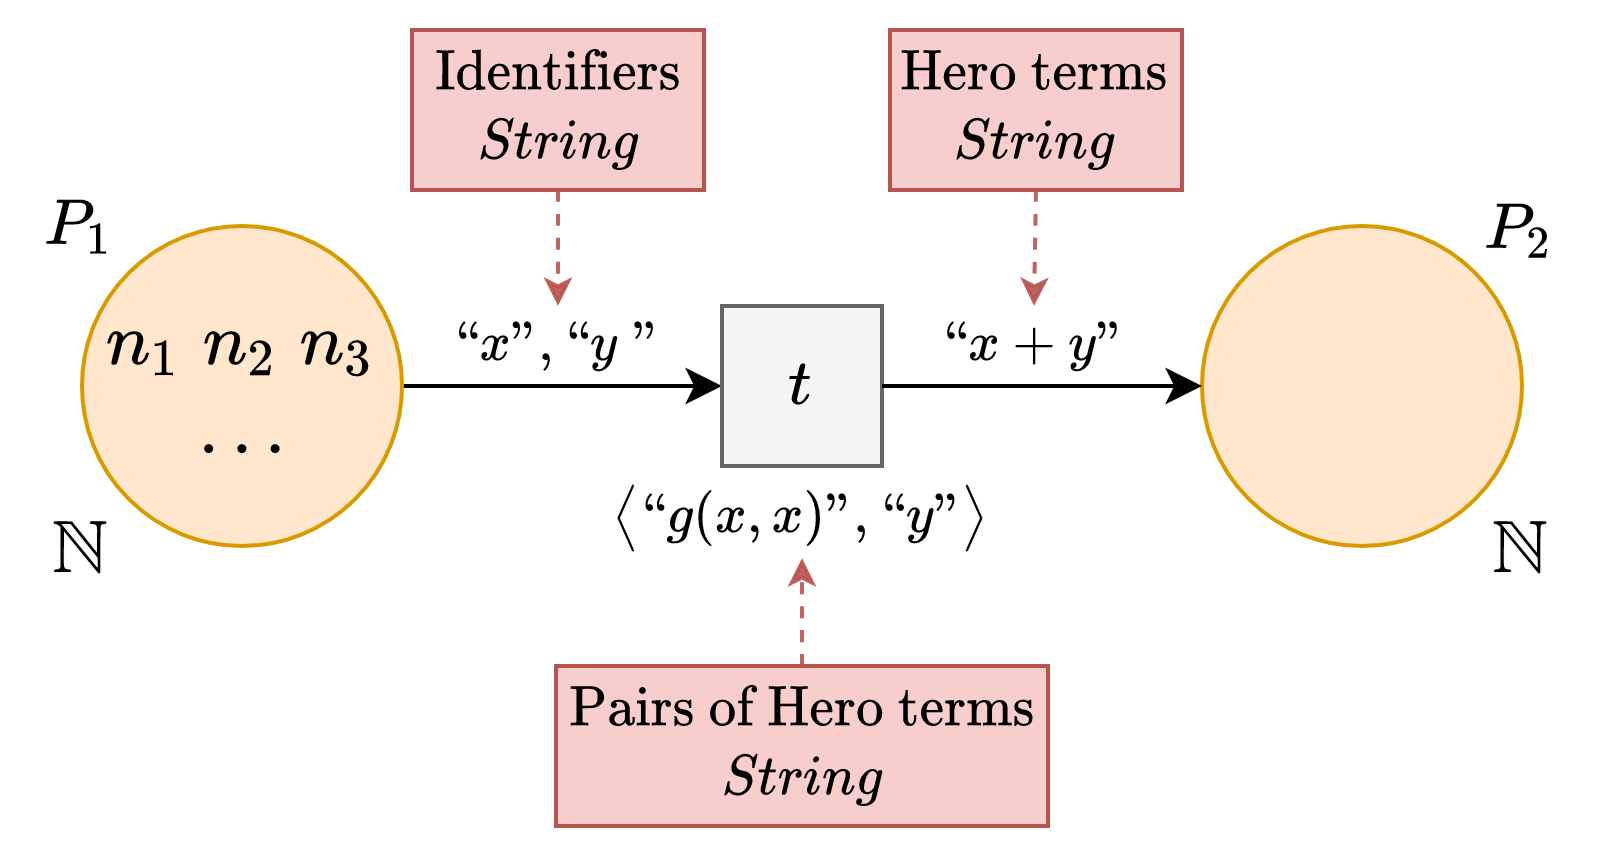
\includegraphics[width=0.80\textwidth]{03integration.png}
    \end{figure}
    \begin{itemize}
        \item Token: set of values (\texttt{Values})
        \item Inbound arc: set of variable identifiers (\texttt{String})
        \item Outbound arc: set of Hero terms (\texttt{String})
        \item Guard: set of pairs of Hero terms (\texttt{String, String})
    \end{itemize}
\end{frame}

\begin{frame}[fragile]{Alpine interpreter modifications}
    \begin{itemize}
        \setlength\itemsep{1.15em}
        \item Input expression:\vspace{\topsep}\begin{itemize}
            \setlength\itemsep{0.45em}
            \item Ex: \texttt{"f(x, g(y)) or y"}
            \item Type: \texttt{String}
        \end{itemize}
        \item Input binding:\vspace{\topsep}\begin{itemize}
            \setlength\itemsep{0.45em}
            \item Ex: \texttt{\{"f" -> and, "g" -> not, "x" -> true, "y" -> false\}}
            \item Type: \texttt{[String: Value]}
        \end{itemize}
        \item Output: evaluation of the expression after substitutions\vspace{\topsep}\begin{itemize}
            \setlength\itemsep{0.45em}
            \item Ex: \texttt{true}
            \item Type: \texttt{Value}
        \end{itemize}
    \end{itemize}
\end{frame}

\begin{frame}[fragile]{Evaluation (1/2)}
    \begin{enumerate}
        \setlength\itemsep{1.15em}
        \item Parse the input expression into an untyped AST\vspace{\topsep}\begin{itemize}
            \setlength\itemsep{0.45em}
            \item \texttt{"f"}, \texttt{"g"}, \texttt{"x"} and \texttt{"y"} are \texttt{Ident} nodes
        \end{itemize}
      \item Substitute the \texttt{Ident} nodes with AST nodes extracted from values
      \item Create the scopes and symbols to be associated with the AST nodes
      \item Bind symbols to their respective scope
      \item Find constraints over symbol types and solve them
      \item Evaluate the typed AST with the corresponding evaluation contexts
    \end{enumerate}
\end{frame}

\begin{frame}[fragile]{Evalution (2/2)}
    \begin{itemize}
        \setlength\itemsep{1.15em}
        \item \texttt{Value}'s type can be a:\vspace{\topsep}\begin{itemize}
            \setlength\itemsep{0.45em}
            \item \underline{Built-in one}: \texttt{Bool}, \texttt{Int}, \texttt{Real}, \texttt{String}, \texttt{([Any]) -> Any}
            \item \underline{Tuple}: \texttt{(Tuple, [Value])}
            \item \underline{Func}: \texttt{(Func, EvaluationContext)}
        \end{itemize}
      \item \texttt{Tuple} and \texttt{Func} are \textbf{AST nodes}, associated with a \textbf{module}, \textbf{symbols} and \textbf{scopes}
    \end{itemize}
    \begin{figure}
        \centering
        
\includegraphics[width=0.17\textwidth]{04scope.png}
    \end{figure}
\end{frame}

\begin{frame}[fragile]{Difficulties}
    \begin{itemize}
        \setlength\itemsep{1.05em}
        \item Little to no experience with Swift
        \item At first no clear understanding of the different sub-steps
        \item Explored up some bad leads (e.g. making \texttt{Scope}, \texttt{Symbol} and every AST nodes conform to
          \texttt{NSCopying})
        \item The evaluation context maps symbols to values, while the \texttt{runSema()} part works with scopes and
          symbols
        \item The module associated with scopes and every AST nodes was being deinitialized after the evaluation
    \end{itemize}
    \begin{figure}
        \centering
        
\includegraphics[width=0.17\textwidth]{05deinit.png}
    \end{figure}
\end{frame}

\begin{frame}[fragile]{Operational Hero net interpreter}
    \begin{figure}
        \centering
        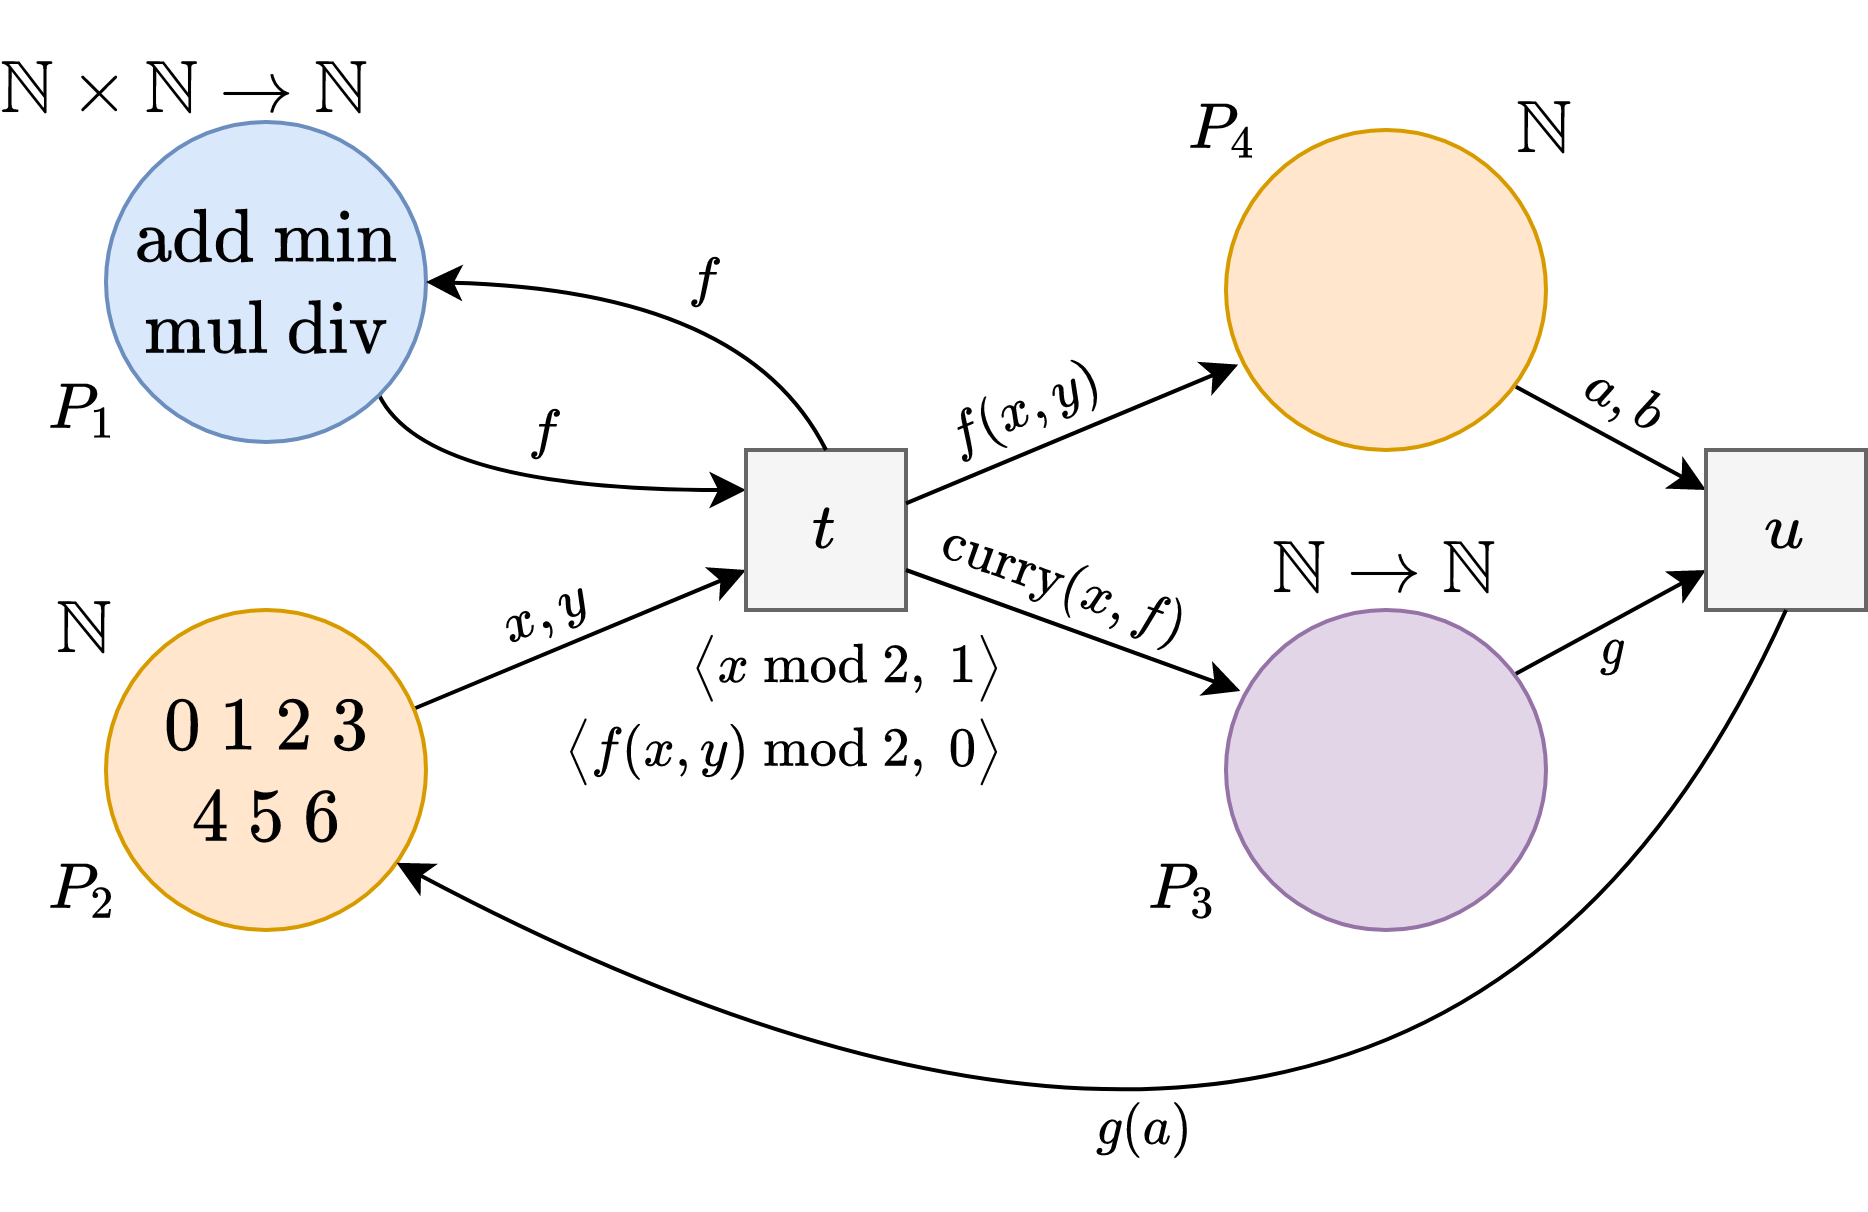
\includegraphics[width=1.0\textwidth]{06heronetexample.png}
    \end{figure}
\end{frame}

\section{Efficient Hero net interpreter}

\begin{frame}[fragile]{MFDD bindings}
    \begin{figure}
        \centering
        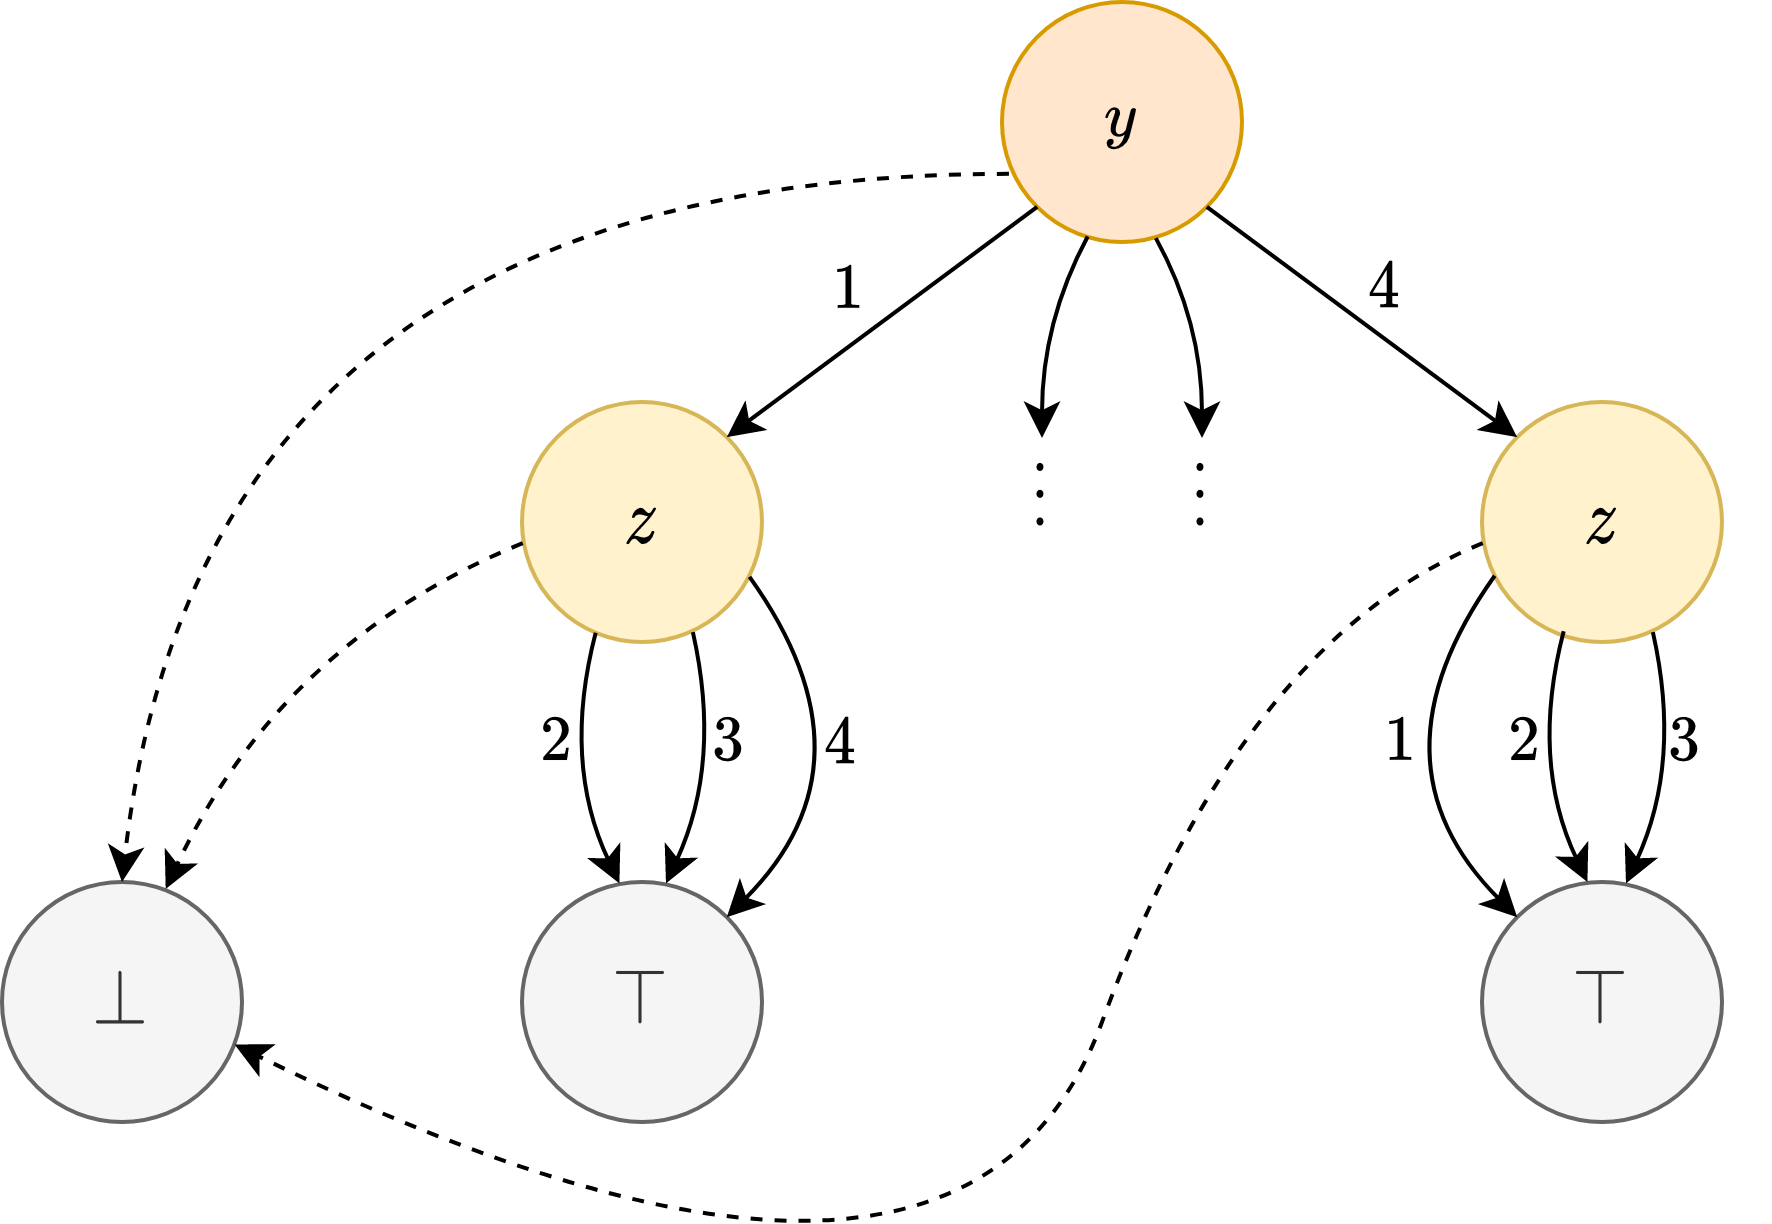
\includegraphics[width=1.0\textwidth]{07mfddold.png}
    \end{figure}
\end{frame}

\begin{frame}[fragile]{MFDD bindings: new method (1/2)}
    \begin{figure}
        \centering
        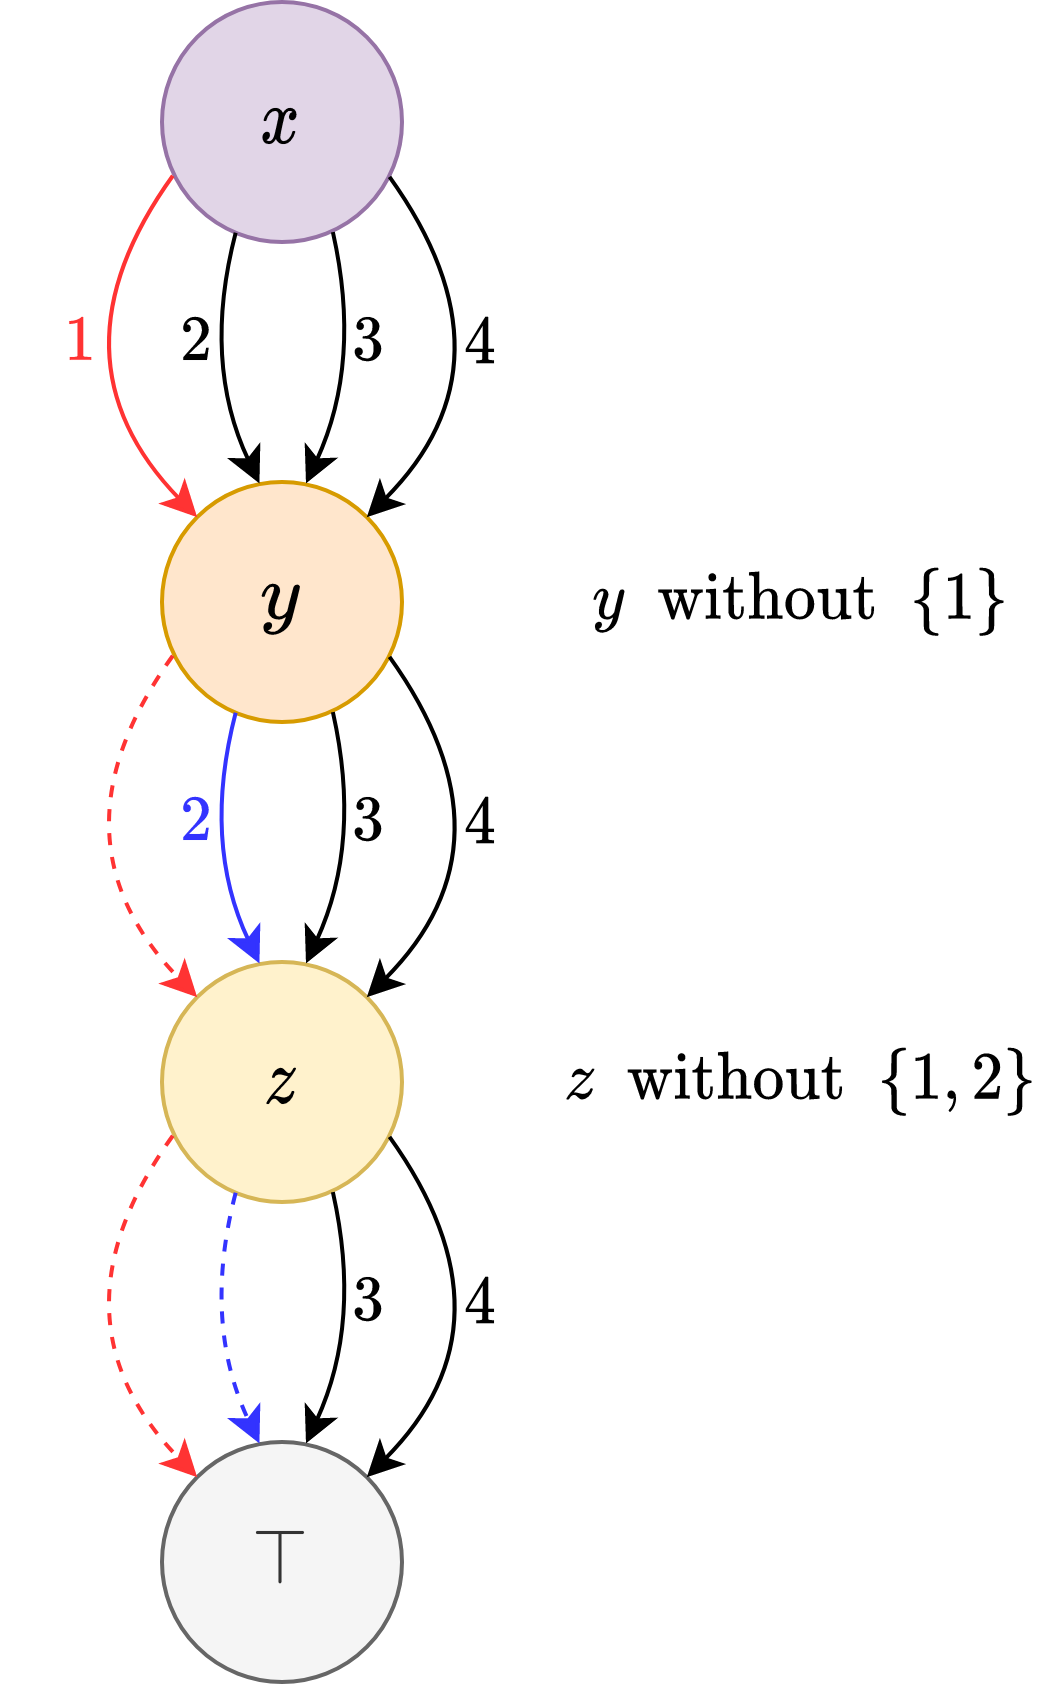
\includegraphics[width=0.45\textwidth]{08mfddnew.png}
    \end{figure}
\end{frame}

\begin{frame}[fragile]{MFDD bindings: new method (2/2)}
    \begin{figure}
        \centering
        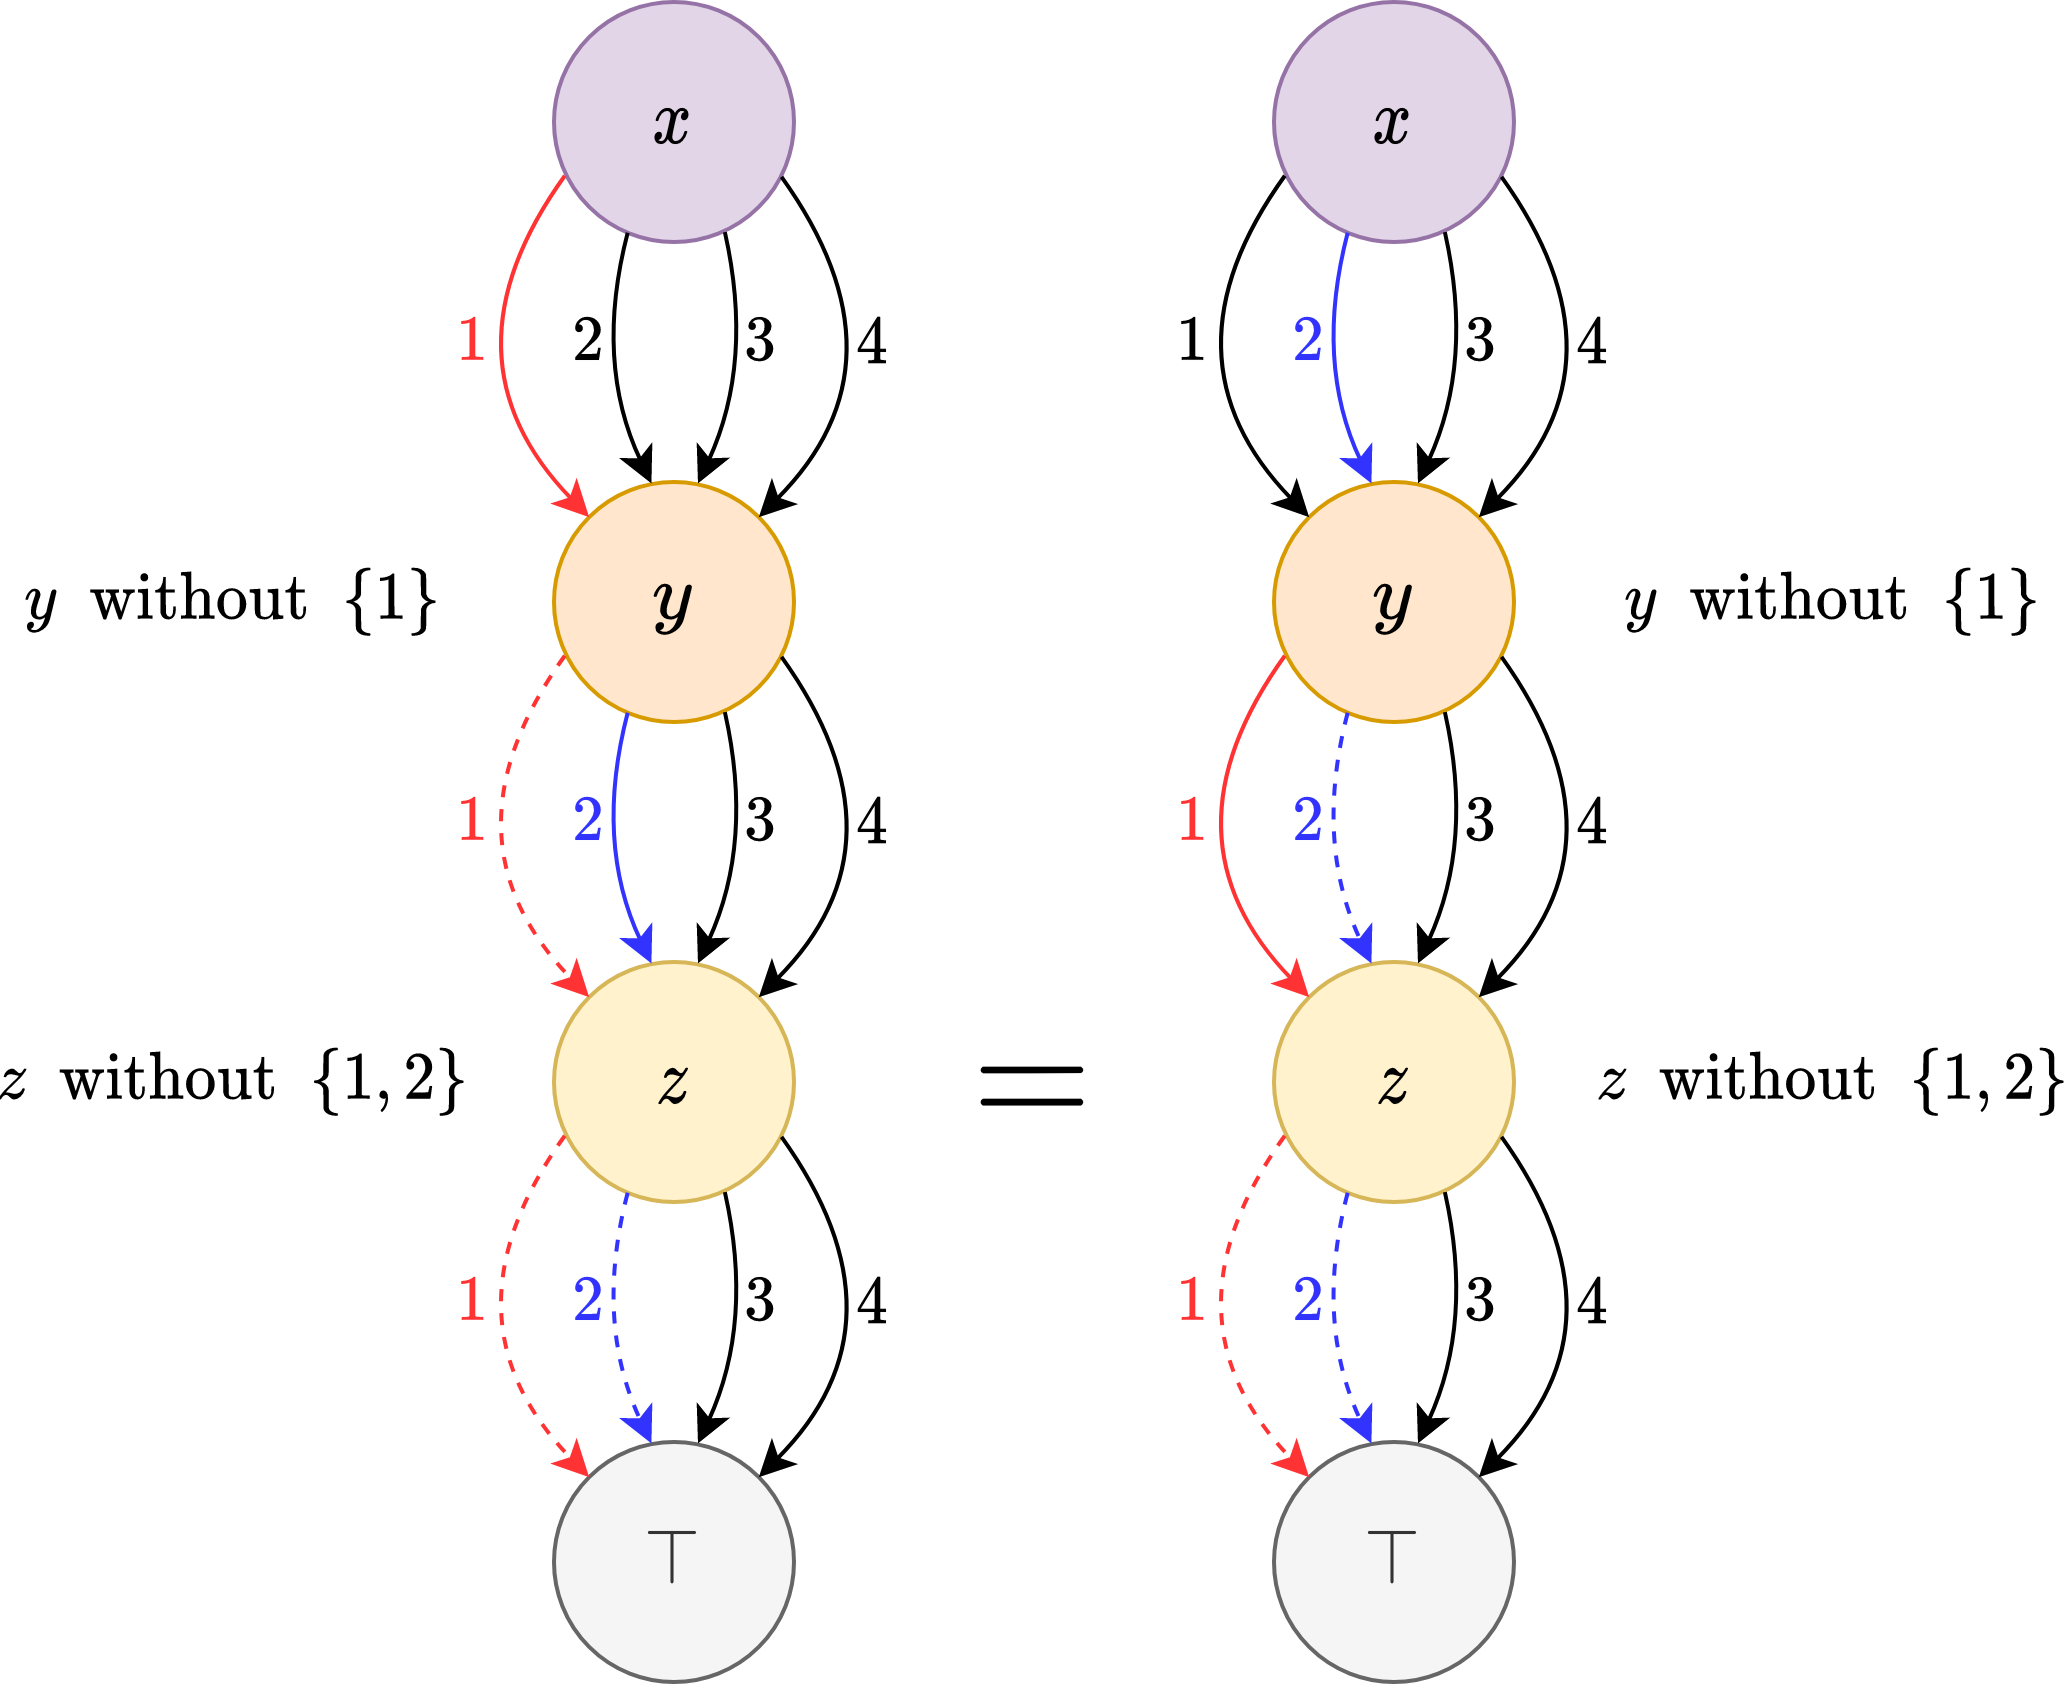
\includegraphics[width=0.9\textwidth]{09mfddcache.png}
    \end{figure}
\end{frame}

\begin{frame}[fragile]{MFDD: fusion}
  \begin{algorithm}[H]
    \DontPrintSemicolon
    \SetKwInOut{Input}{Input}\SetKwInOut{Output}{Output}
    \SetKwFunction{Ffusion}{fusion}
    \SetKwProg{Fn}{Function}{:}{}    
    \Input{lhs, rhs}
    \Output{Fusion of lhs and rhs}
    \BlankLine

    \Fn{\Ffusion{$lhs$, $rhs$}}{
      \If{$\text{lhs} = \text{one}$}
      {
          \KwRet rhs
      }
      \ElseIf{$\text{rhs} = \text{one}$}
      {
          \KwRet lhs
      }

      \If{$\text{lhs.key} > \text{rhs.key}$}
      {
          \KwRet fusion(rhs, lhs)
      }
      \KwRet node(\hspace{-2em}\newline
            \hspace*{0.65em} lhs.key,\newline
            \hspace*{0.65em} lhs.take.mapValue \{ fusion(\$0, rhs) \}\newline
            \hspace*{0.65em} zero)
    }
  \caption{Combining MFDDs representing permutations}
  \end{algorithm}
\end{frame}

\begin{frame}[fragile]{Guards: simple strategy}
    \begin{figure}
        \centering
        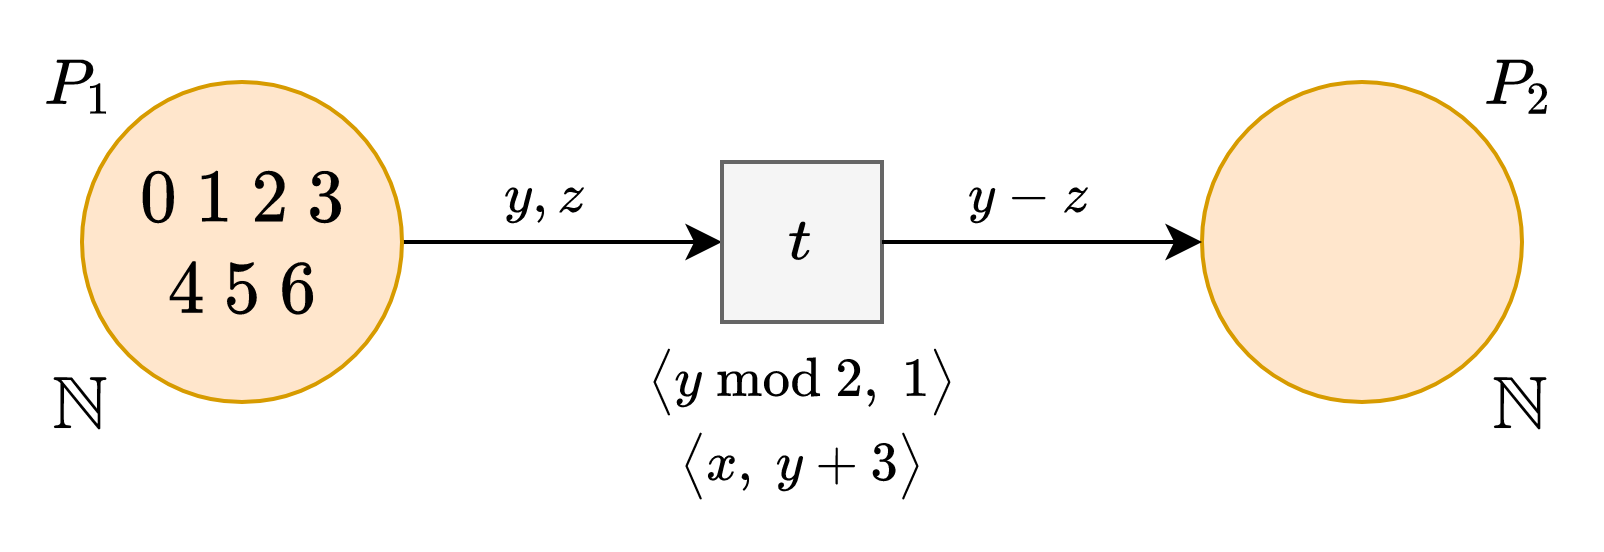
\includegraphics[width=1.0\textwidth]{guards.png}
    \end{figure}
    \begin{enumerate}
        \setlength\itemsep{1.15em}
        \item Explore the MFDD until we find all the needed variables
        \item Evaluate the two expressions with the resulting binding
        \item Prune node if not equal
    \end{enumerate}
\end{frame}

\begin{frame}[fragile]{Guards: example}
    \begin{figure}
        \centering
        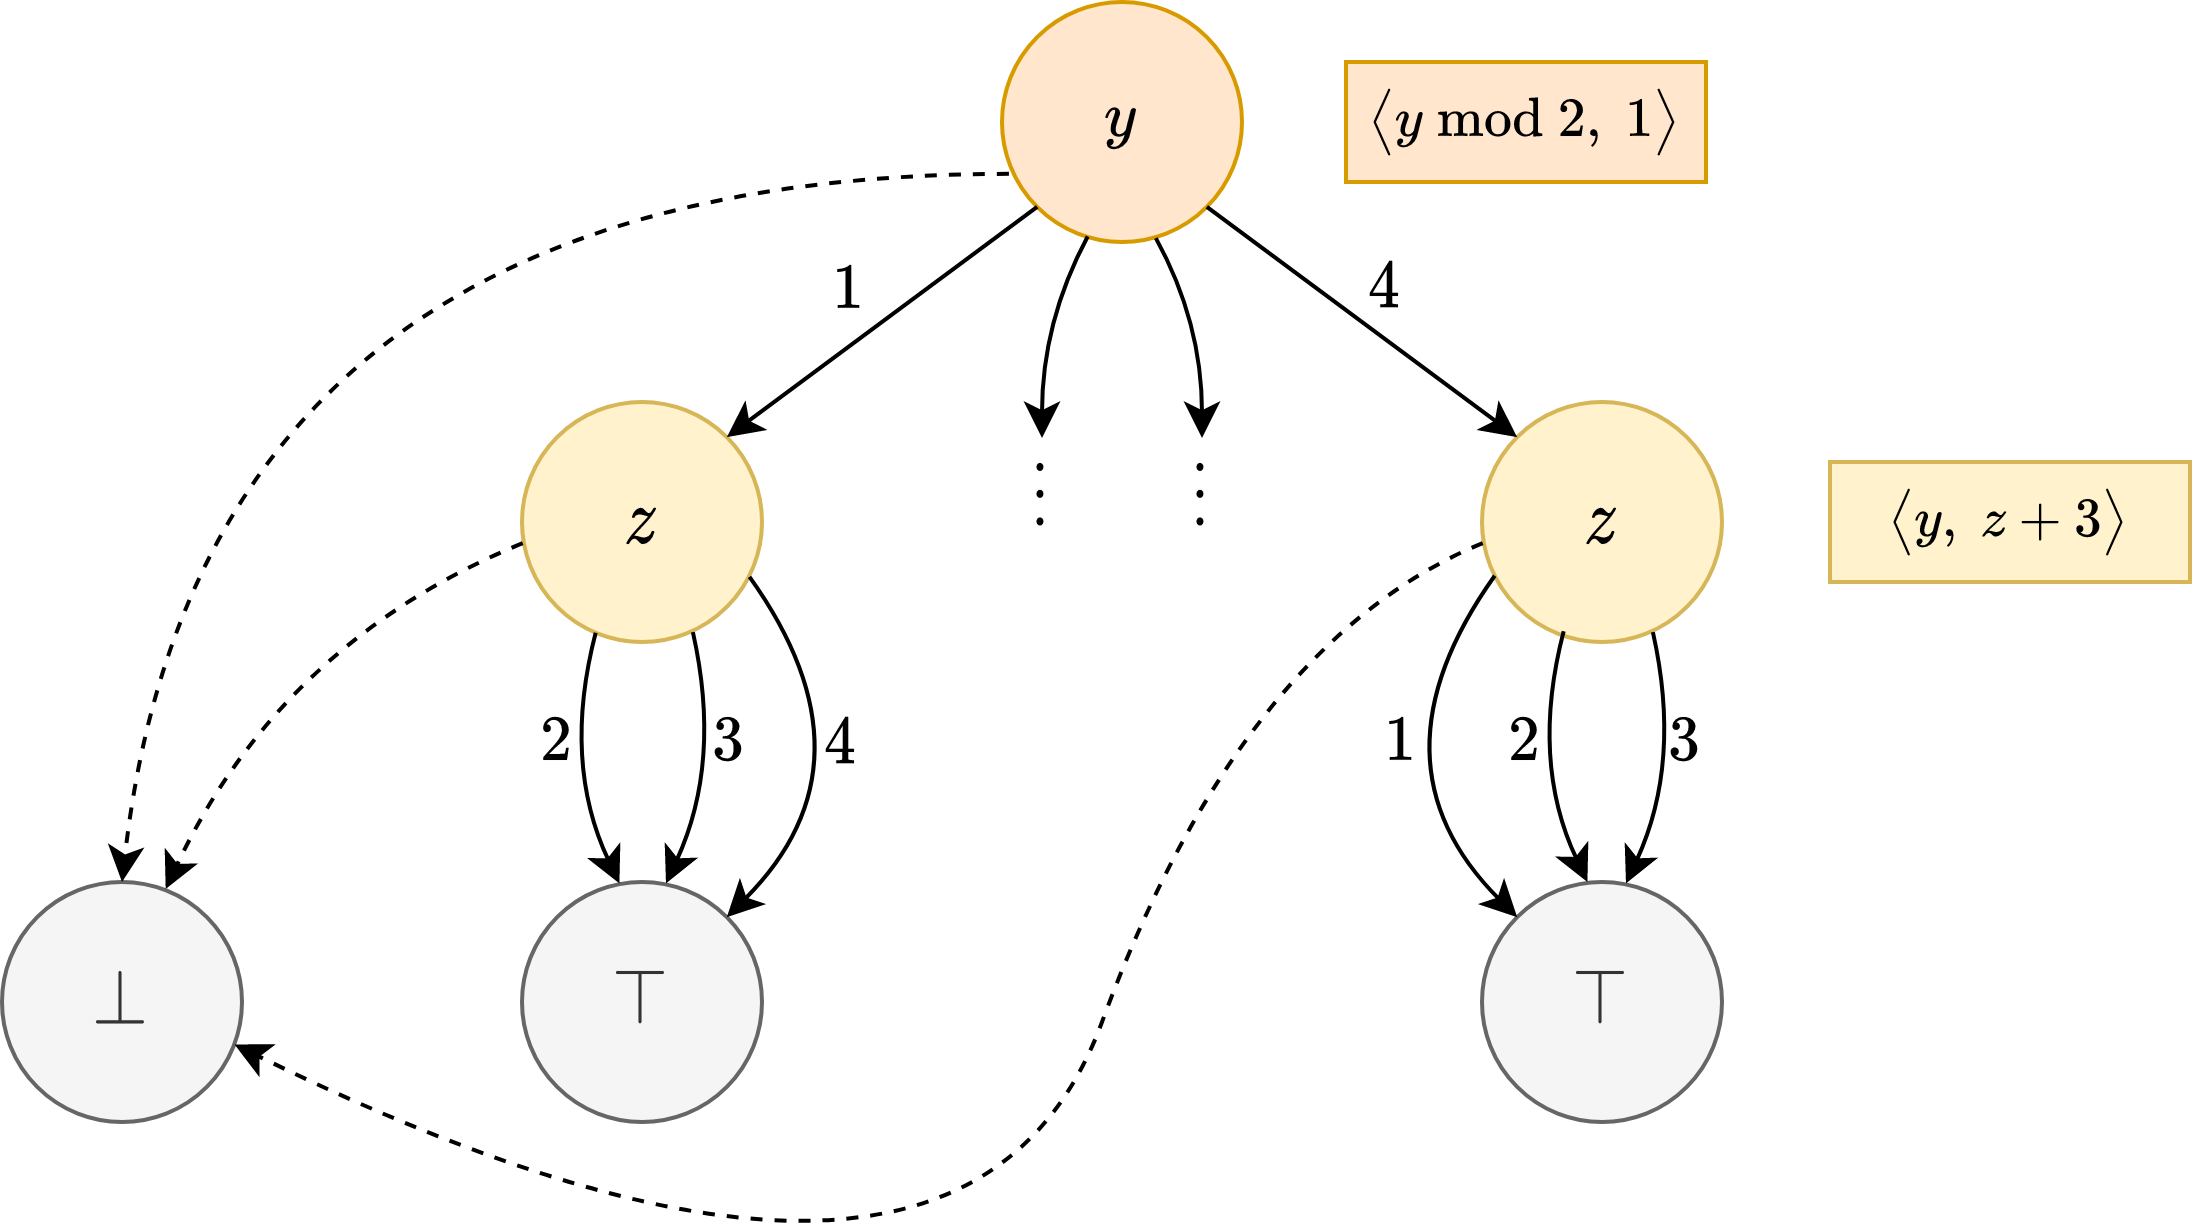
\includegraphics[width=1.0\textwidth]{guardsex.png}
    \end{figure}
\end{frame}

\begin{frame}[fragile]{Several improvements}
    \begin{itemize}
        \setlength\itemsep{1.15em}
        \item Add a cache mechanism to \vspace{\topsep}\begin{itemize}
            \setlength\itemsep{0.45em}
            \item Fusion
            \item Guard filtering
            \item Alpine evalution
        \end{itemize}
        \item Variable and guard ordering\vspace{\topsep}\begin{itemize}
            \setlength\itemsep{0.45em}
            \item Variables appearing in guards are put at the top
            \item Of these variables, those in the guards with the smallest number of different variables have the
              smallest index
            \item Guards featuring the fewest number of variables with the smallest indexes are checked first 
        \end{itemize}
    \end{itemize}
\end{frame}

\begin{frame}[fragile]{Benchmark: lots of conditions (1/2)}
    \begin{figure}
        \centering
        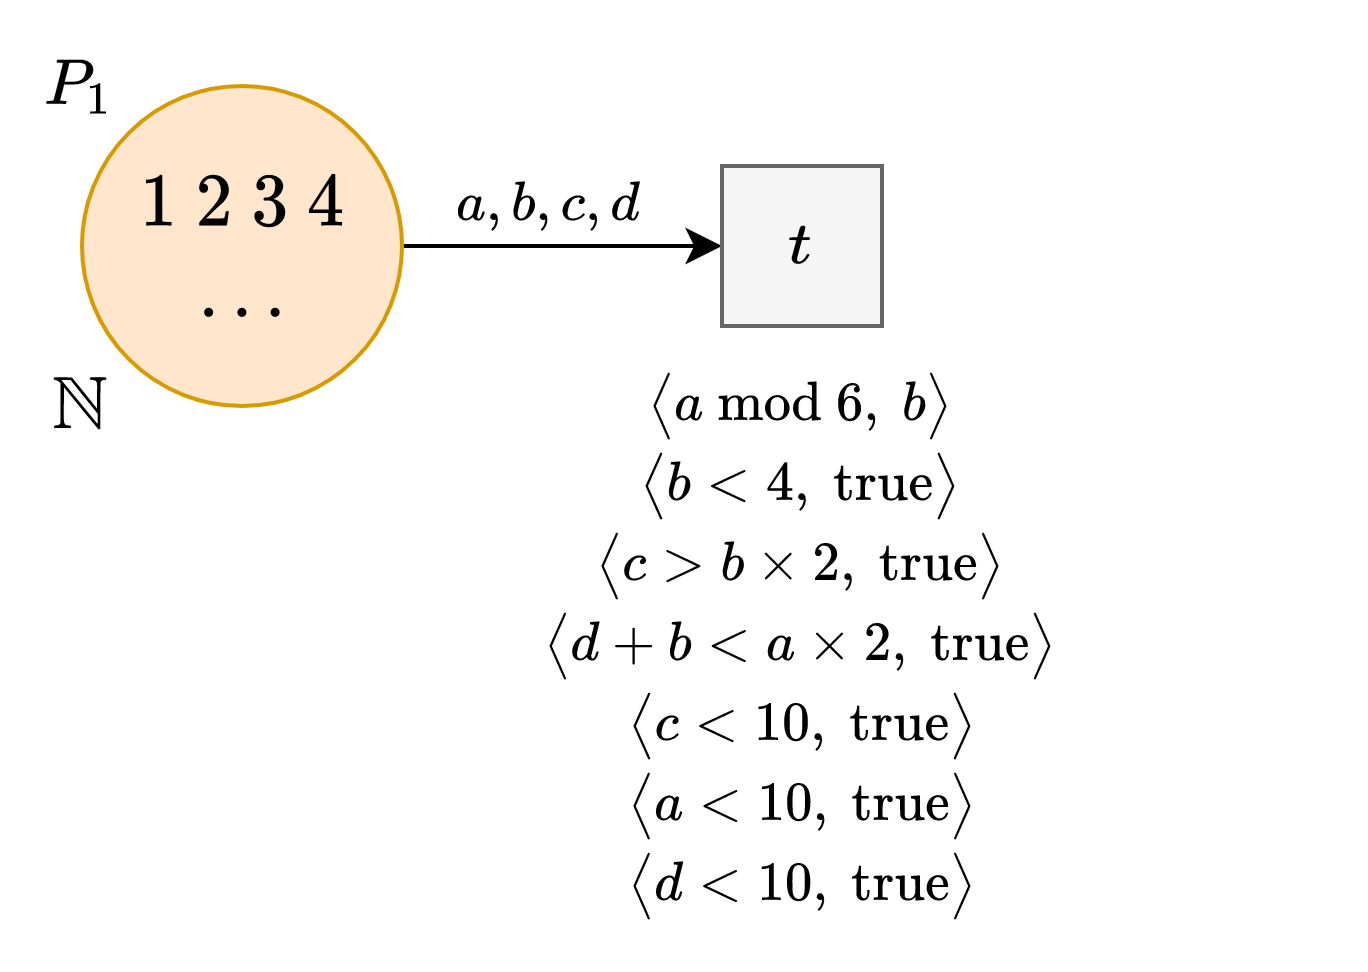
\includegraphics[width=1.0\textwidth]{lotsc.png}
    \end{figure}
\end{frame}

\begin{frame}[fragile]{Benchmark: lots of conditions (2/2)}
    \begin{figure}
        \centering
        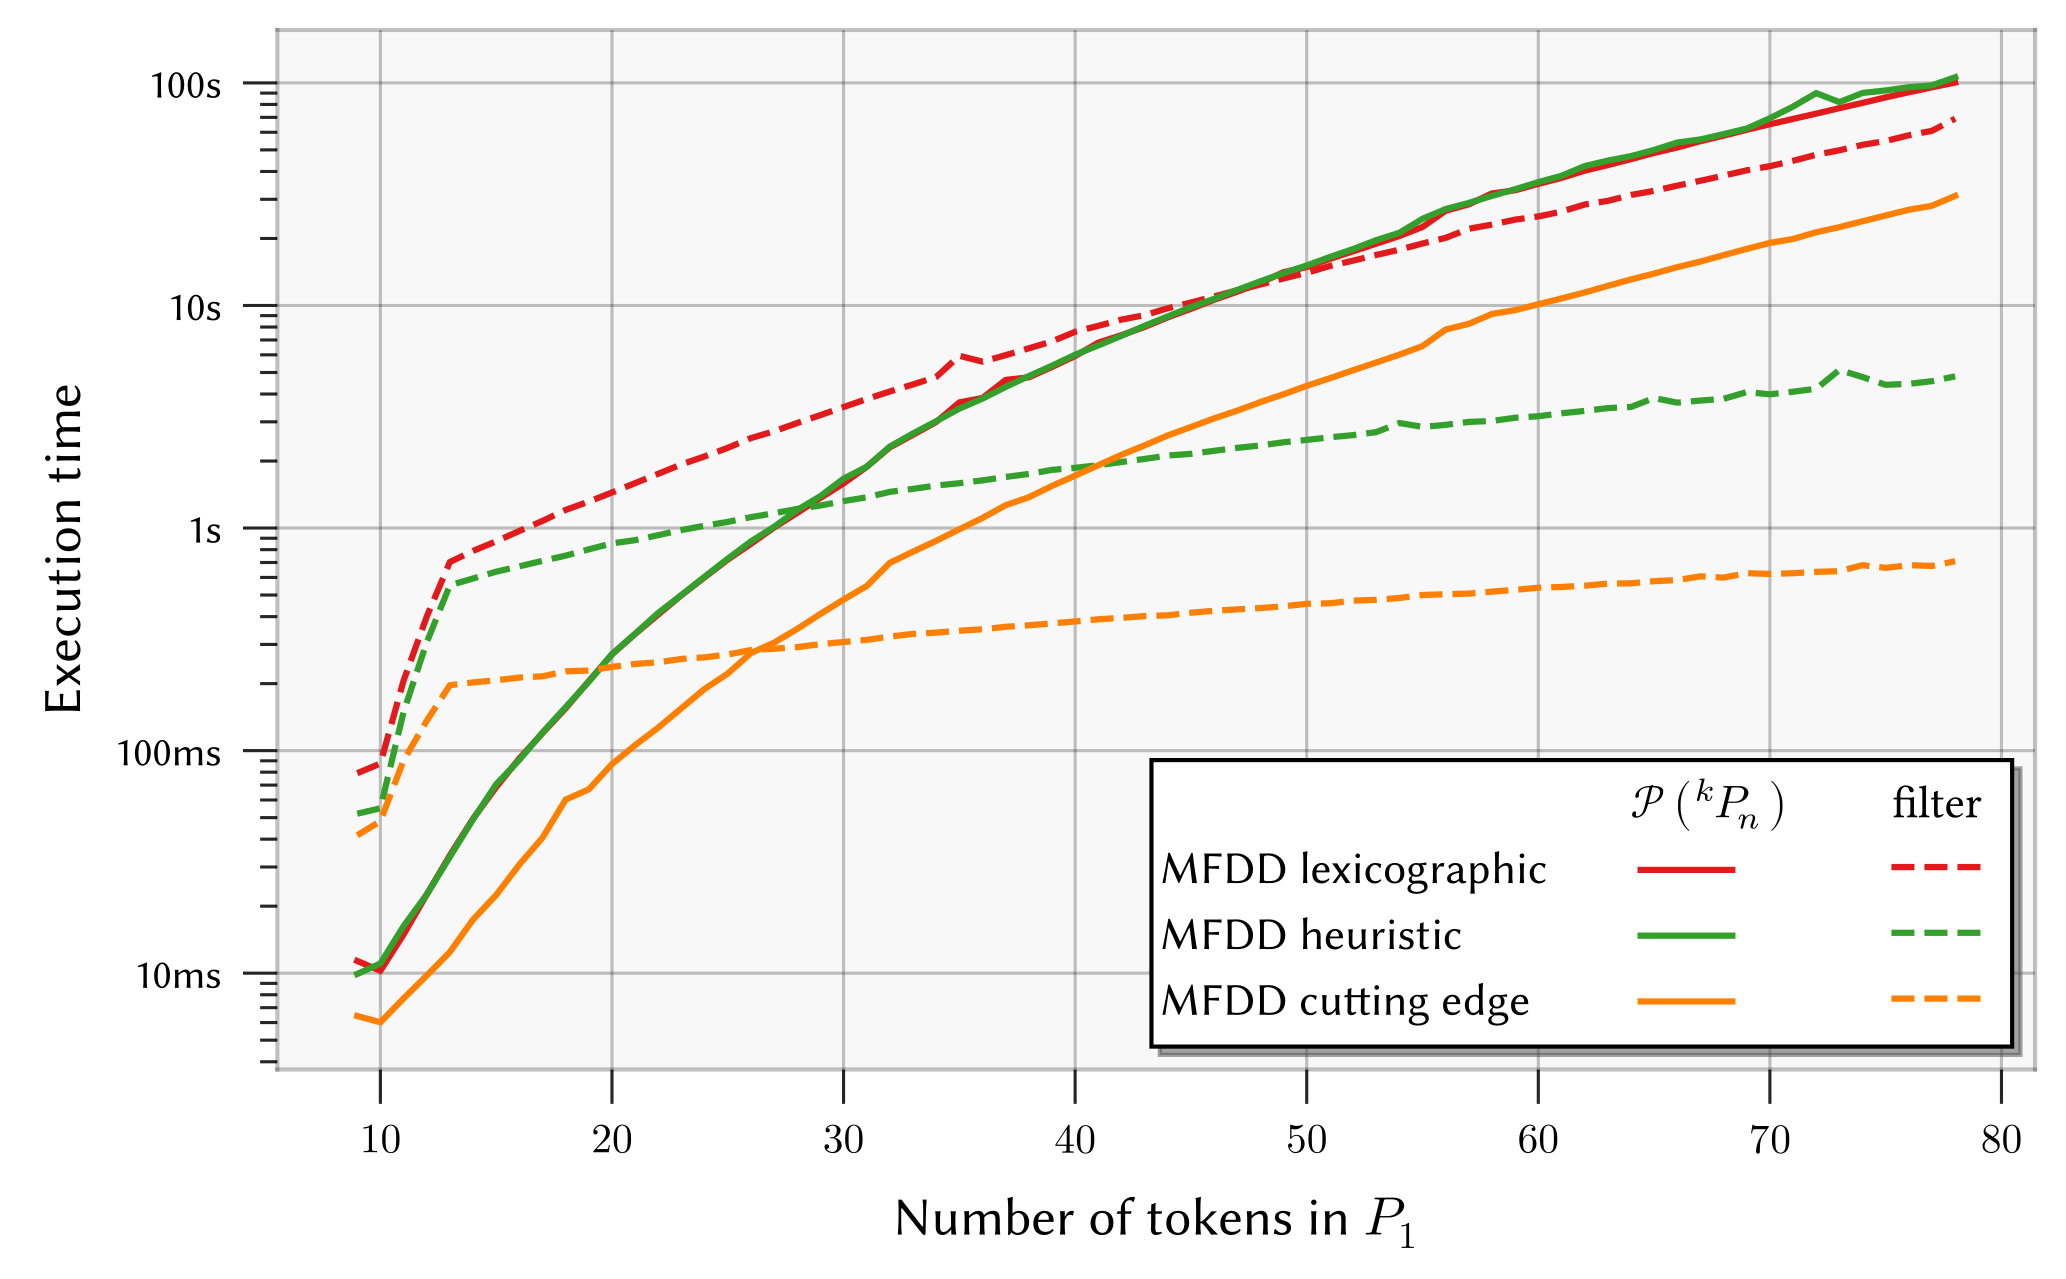
\includegraphics[width=1.0\textwidth]{benchlotsc.png}
    \end{figure}
\end{frame}

\begin{frame}[fragile]{Benchmark: simple Hero net (1/2)}
    \begin{figure}
        \centering
        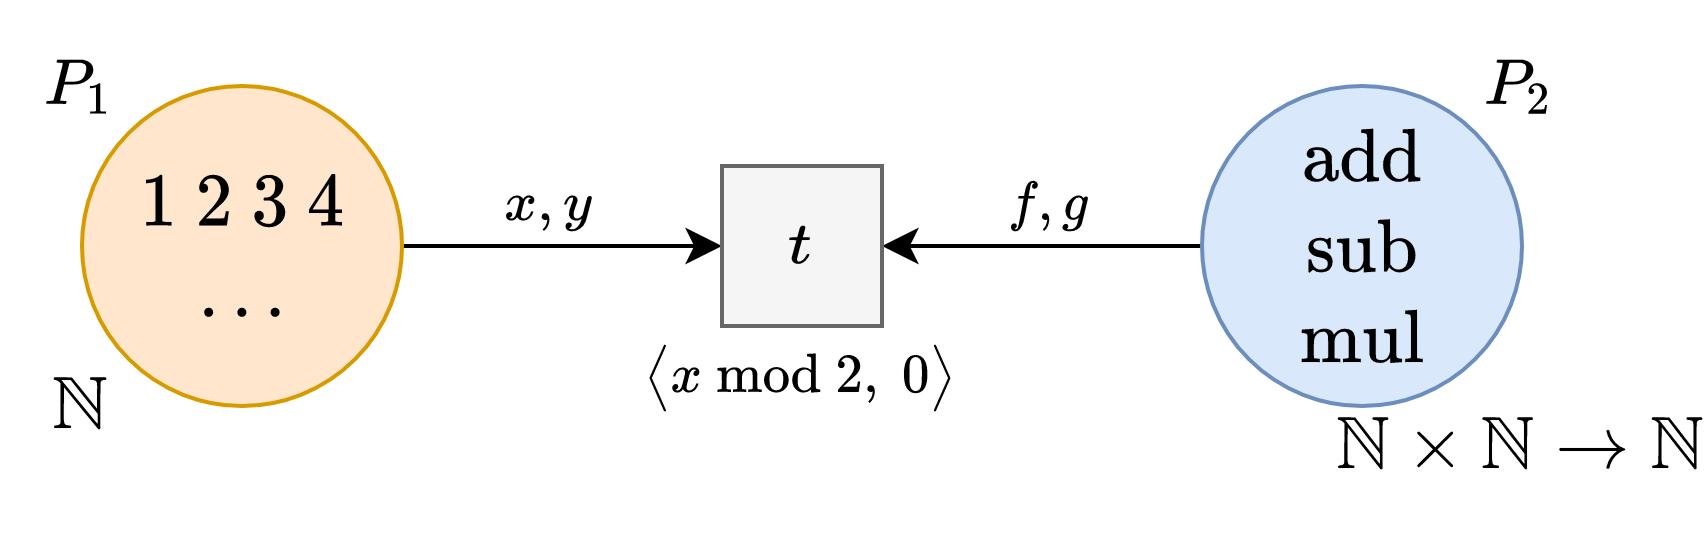
\includegraphics[width=1.0\textwidth]{brute.png}
    \end{figure}
\end{frame}

\begin{frame}[fragile]{Benchmark: simple Hero net (2/2)}
    \begin{figure}
        \centering
        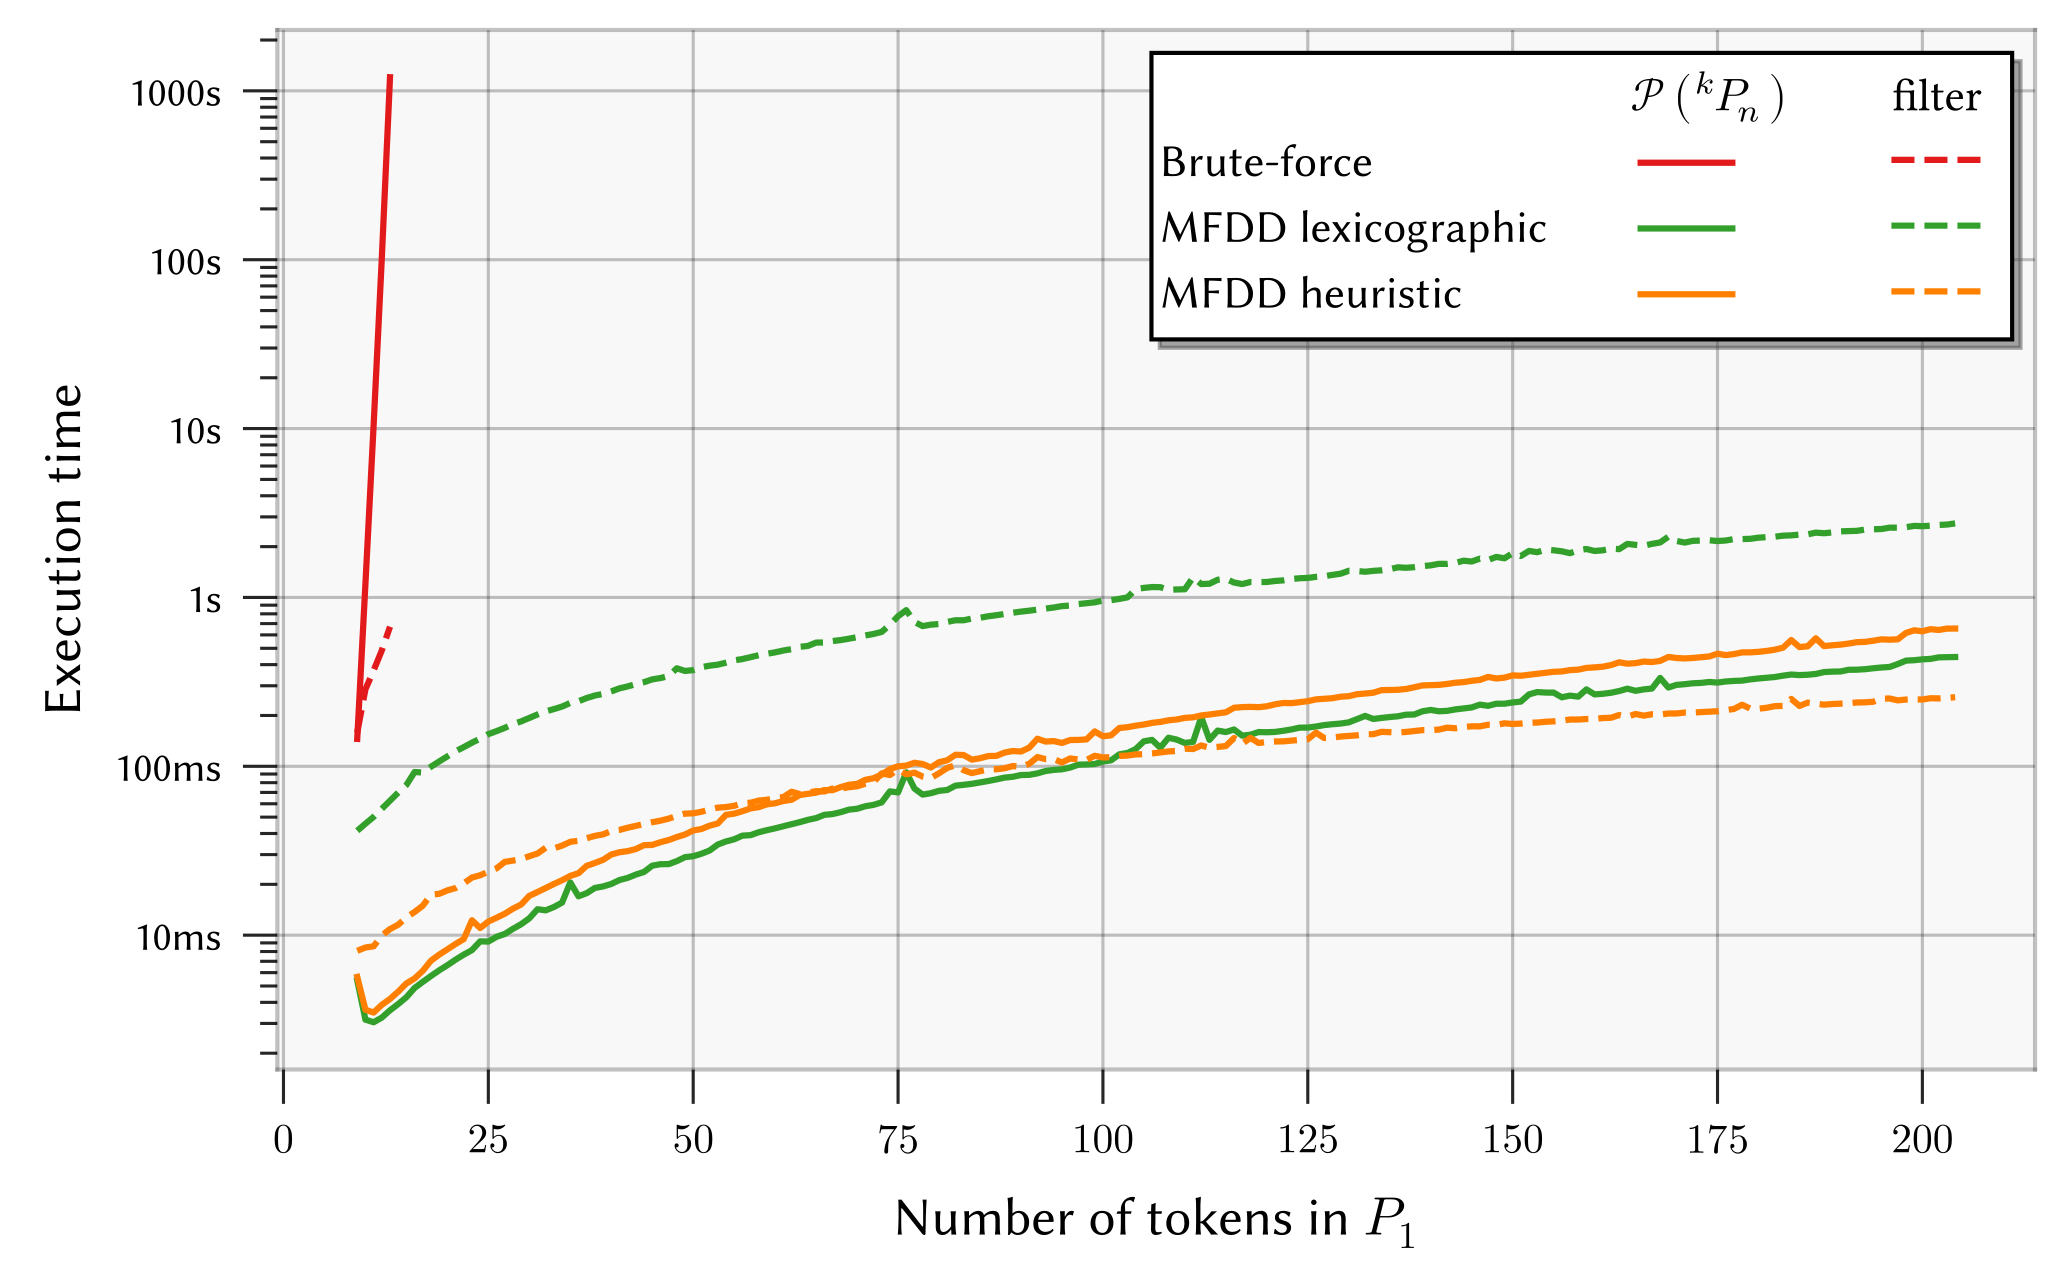
\includegraphics[width=1.0\textwidth]{benchbrute.png}
    \end{figure}
\end{frame}

\begin{frame}[fragile]{Benchmark: in order (1/2)}
    \begin{figure}
        \centering
        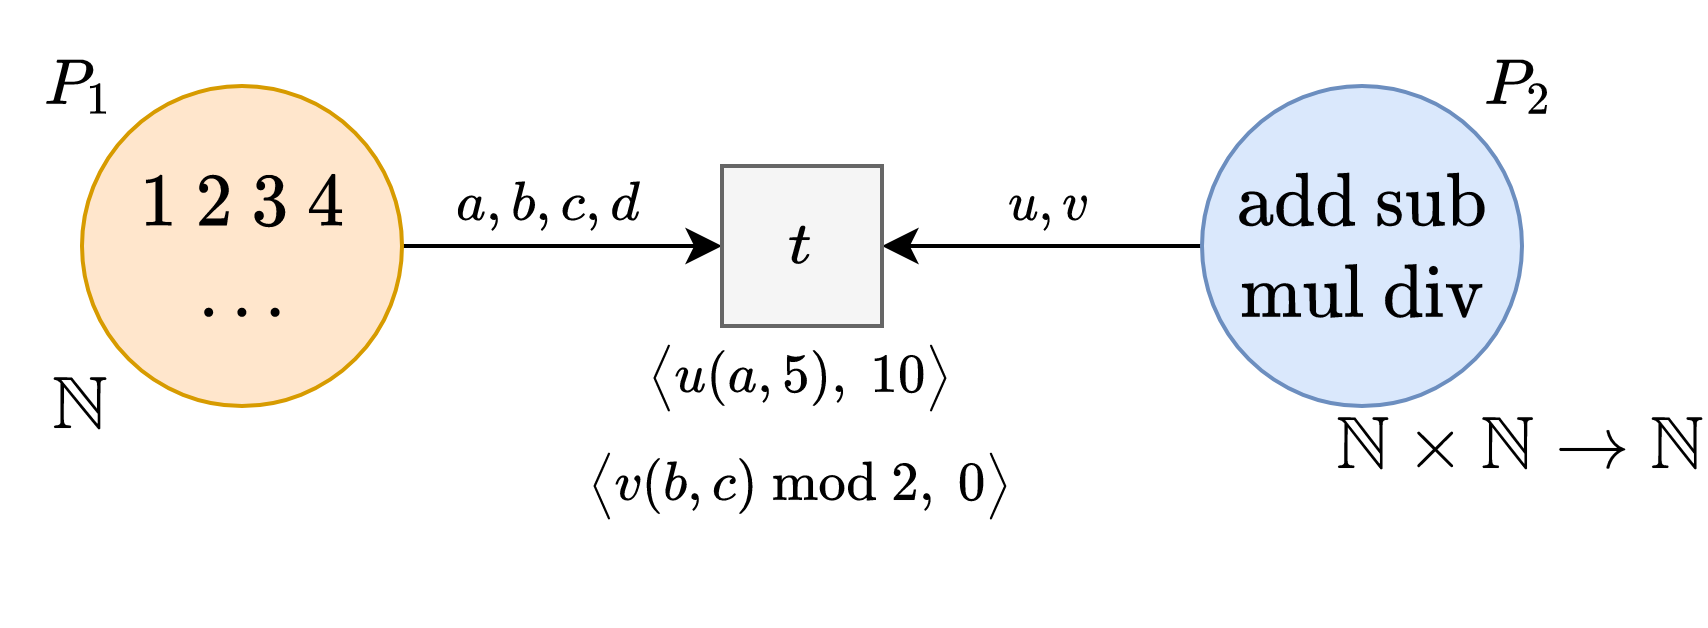
\includegraphics[width=1.0\textwidth]{5v.png}
    \end{figure}
\end{frame}

\begin{frame}[fragile]{Benchmark: in order (2/2)}
    \begin{figure}
        \centering
        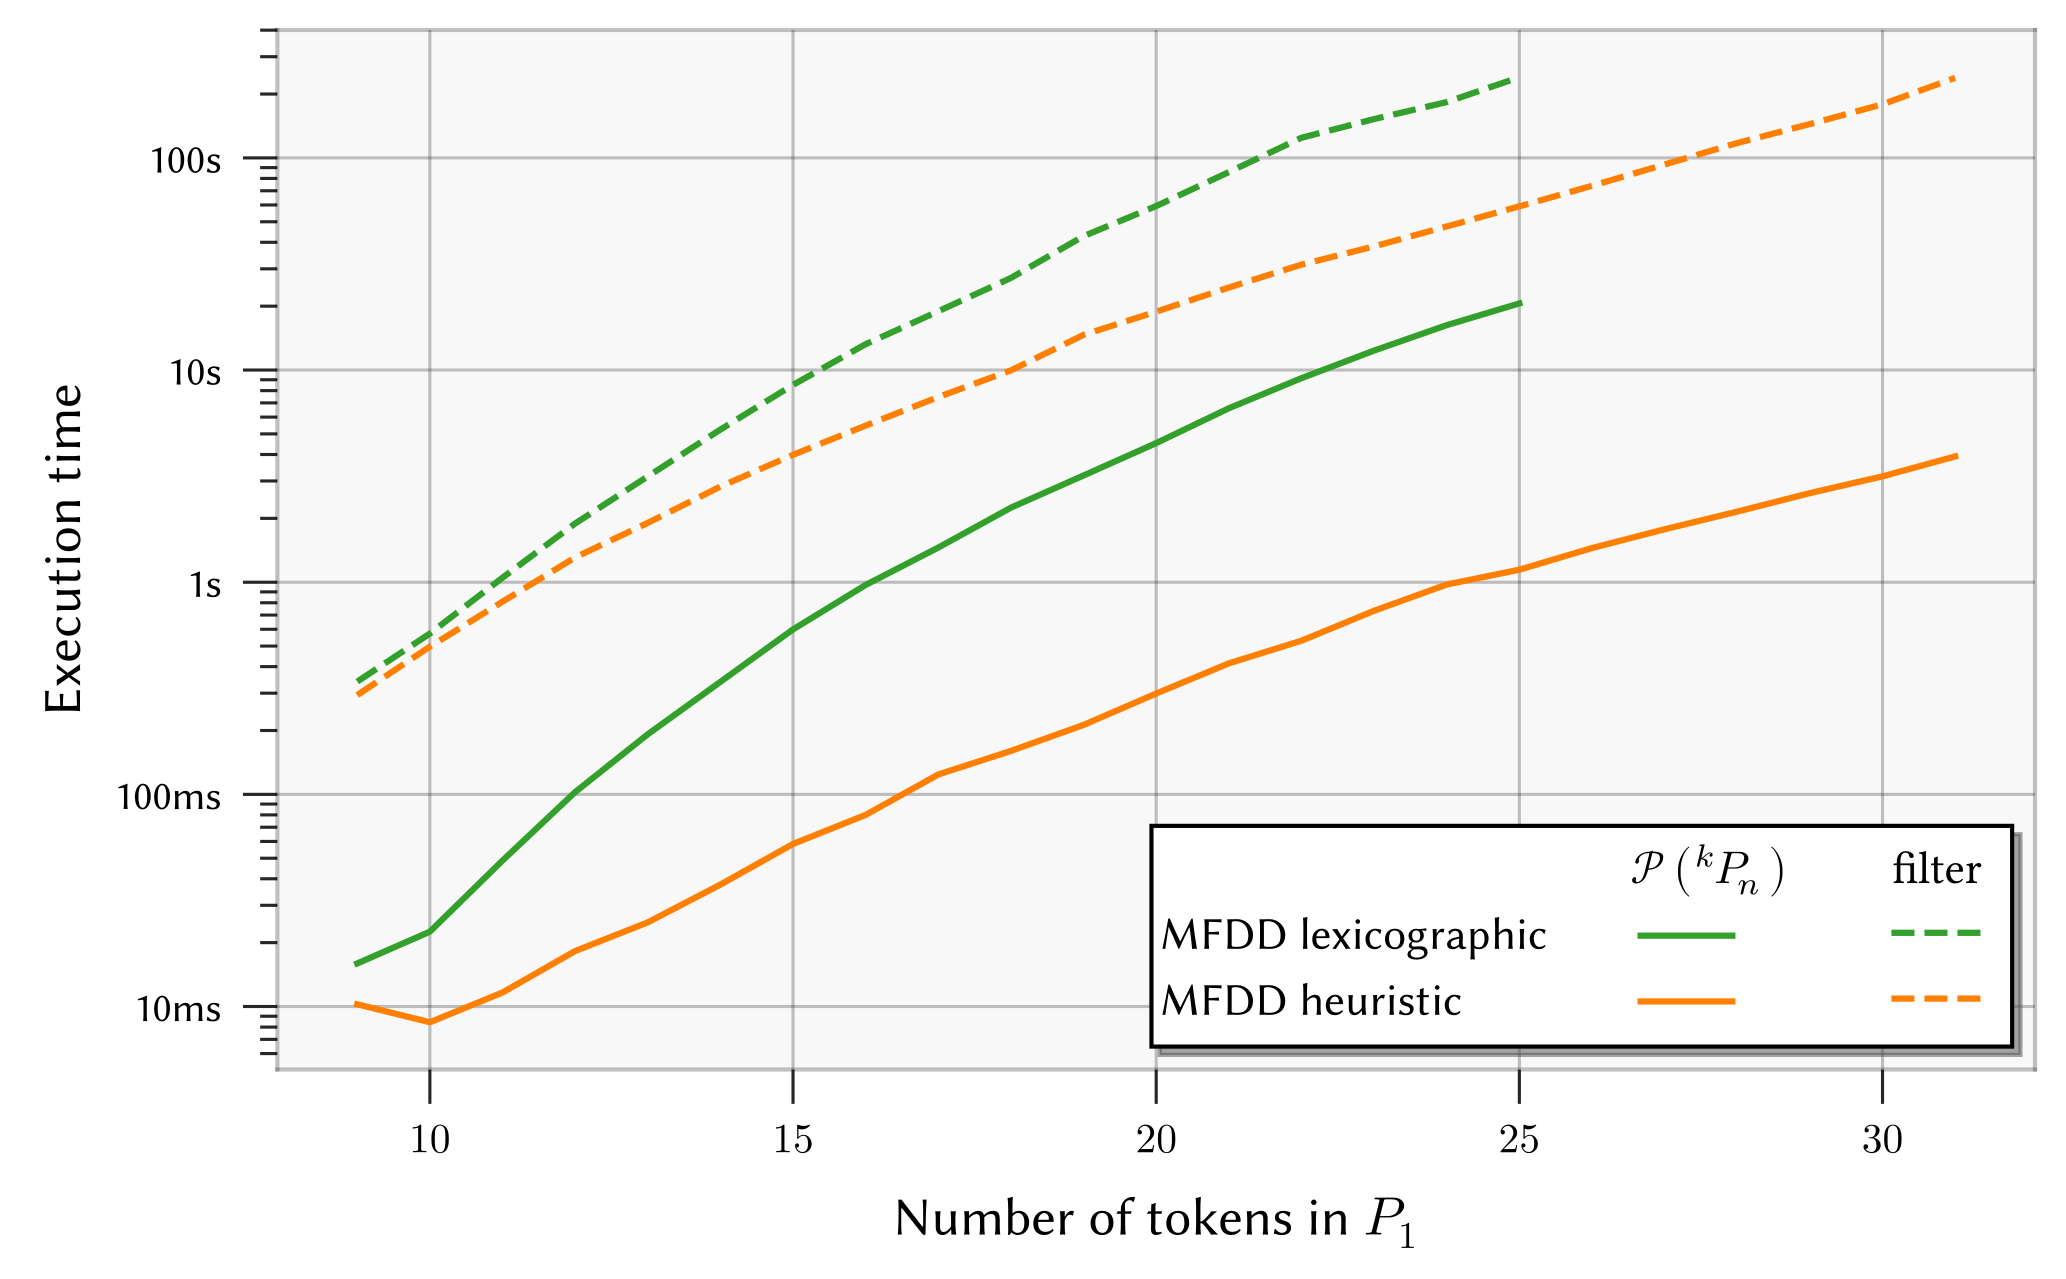
\includegraphics[width=1.0\textwidth]{bench5v.png}
    \end{figure}
\end{frame}

\begin{frame}[fragile]{Benchmark: in disorder (1/2)}
    \begin{figure}
        \centering
        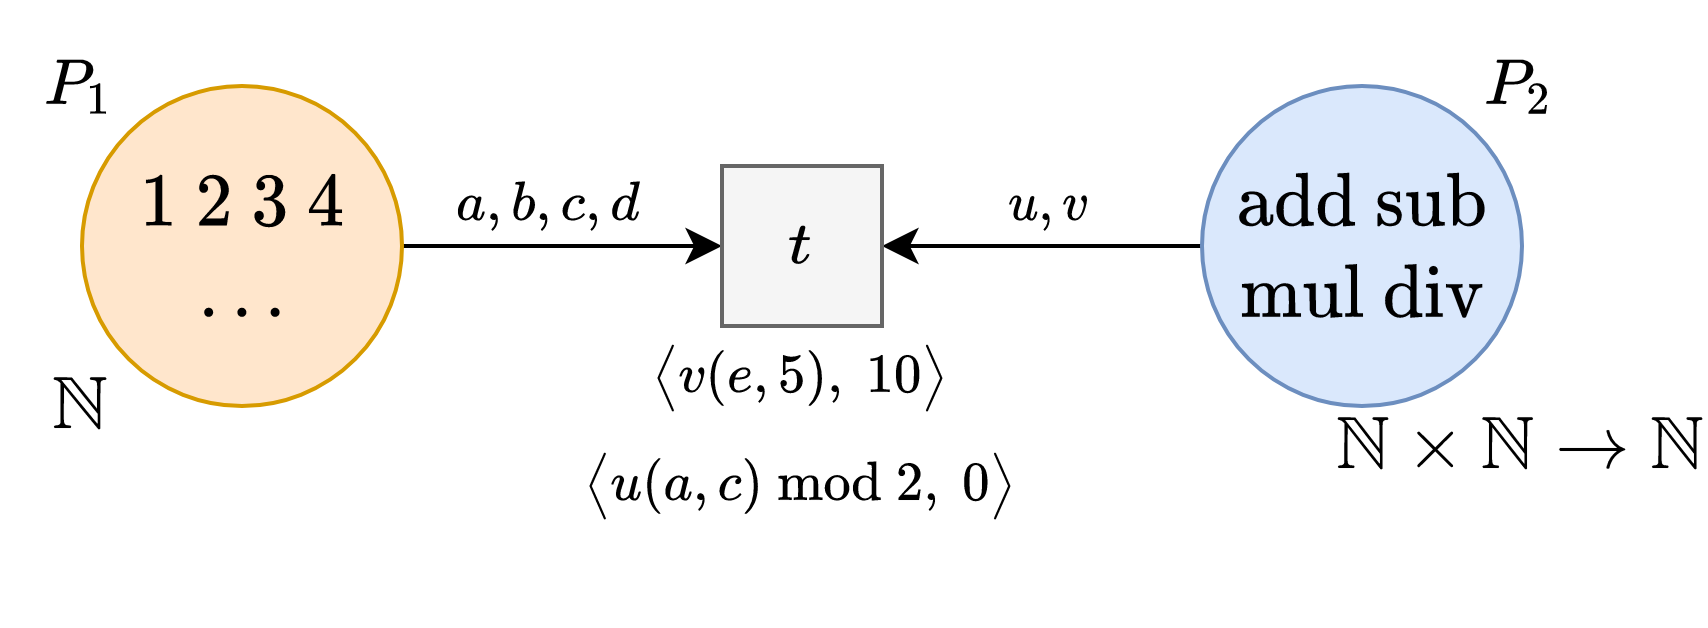
\includegraphics[width=1.0\textwidth]{5v2.png}
    \end{figure}
\end{frame}

\begin{frame}[fragile]{Benchmark: in disorder (2/2)}
    \begin{figure}
        \centering
        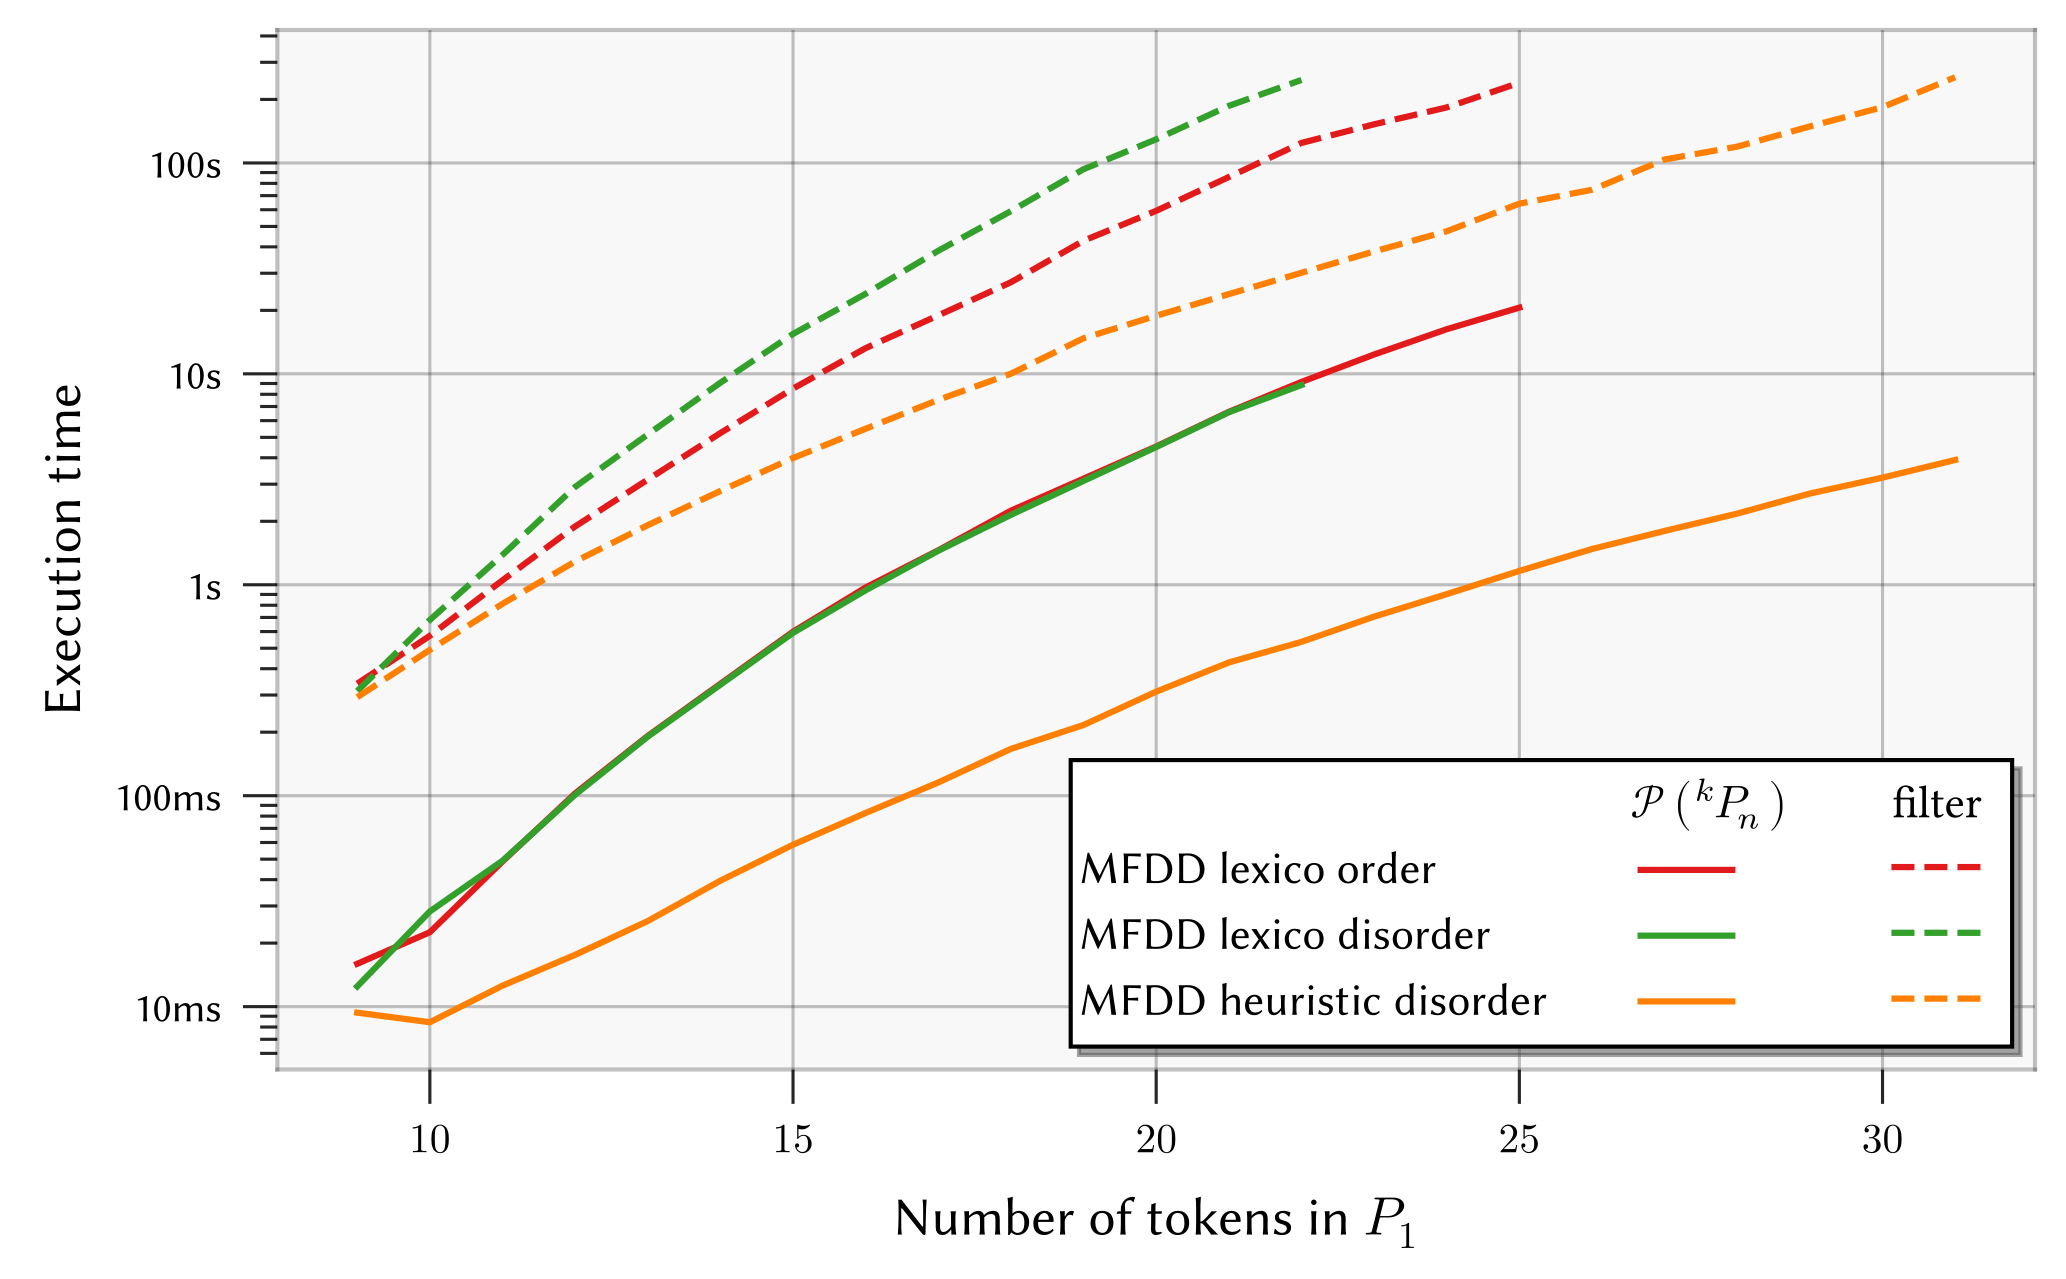
\includegraphics[width=1.0\textwidth]{bench5v2.png}
    \end{figure}
\end{frame}

\begin{frame}[fragile]{There is room for improvement!}
    \begin{itemize}
        \setlength\itemsep{1.15em}
        \item Clean the code
        \item Better caching mechanisms (especially with Alpine)
        \item Better variable ordering
        \item Better guard filtering (parse ASTs)
        \item Combine MFDD initial construction and guard filtering
    \end{itemize}
\end{frame}

\section{Thank you!}

\end{document}
